\documentclass[11pt,twoside,colorback,accentcolor=tud2c,nopartpage,bigchapter,fleqn,ngerman]{tudreport}
% Für Skripte 11pt-Schrift verwenden (Standard ist 9.5)


% Für Entwurf auf Rechnern ohne installierte TUDdesign-Pakete
% scrreprt kennt keine Schriftgröße 9.5pt
%\documentclass[10pt,twoside,fleqn,ngerman]{scrreprt}


% =================================================================================
% Falls scrreprt anstelle von tudreport gewählt, muss das über diesen Schalter
% mitgeteilt werden!
% =================================================================================

\newif\ifStdClassDraft
\StdClassDraftfalse	% tudreport
%\StdClassDrafttrue		% scrreprt

% =================================================================================



% =================================================================================
% Definitionen aus tudreport-Vorlage
% =================================================================================
\newif\ifTUDmargin
%\TUDmargintrue		% Sehr breiter rechter Rand
\TUDmarginfalse		% Schmaler (normaler) rechter Rand

\ifTUDmargin	% ggf. breiten Rand setzen
  \geometry{marginparsep=4.2mm,marginparwidth=28.64mm}
\fi

\newlength{\longtablewidth}
\setlength{\longtablewidth}{0.7\linewidth}
\addtolength{\longtablewidth}{-\marginparsep}
\addtolength{\longtablewidth}{-\marginparwidth}
% =================================================================================



% =================================================================================
% Hauptdefintionen sind aus Platzgründen ausgelagert
% =================================================================================

% Einbinden wichtiger und weniger wichtiger Pakete
\input{common/includes.tex}

\ifStdClassDraft
	% Diese Pakete nur extra einbinden, wenn NICHT tudreport als Basis.
	\usepackage{amssymb}
	\usepackage{geometry}
\fi


% Einrichten verschiedener Umgebungen, Listing-Formate, etc.
\input{common/setups.tex}


% Nützliche Befehle und Abkürzungen
\input{common/commonmacros.tex}

% =================================================================================



% =================================================================================
% Befehle, die in scrreprt nicht exisiteren werden hier definiert, wenn diese
% Klasse verwendet wird.
% Auch die Seitenränder werden angepasst, so dass es grob wie mit tudreport
% aussieht.
% =================================================================================
\ifStdClassDraft
	\newcommand{\subsubtitle}[1]{}
	\newcommand{\settitlepicture}[1]{}
	\newcommand{\printpicturesize}{}
	\newcommand{\institution}[1]{}
	
	\author{}	% scrreprt erwartet Autor
	
	\geometry{left=20mm, right=15mm, top=15mm, bottom=20mm}
\fi
% =================================================================================



% =================================================================================
% Anpassung Absatzformat
% =================================================================================
% Wenn nur sehr kurze Absätze mit vielen Formeln im Text vorkommen, dann sieht der 
% standardmäßig vorhandene Einzug bei Absatzbeginn etwas unruhig aus. Dann kann
% dieser hier auf Null gesetzt, und dafür der vertikale Abstand zwischen zwei
% Absätzen etwas vergrößert werden.
%
\setlength{\parindent}{0mm}
\setlength{\parskip}{1ex}
% =================================================================================




% =================================================================================
% Texte für den Titel und die Rückseite des Titels vorgeben
% =================================================================================
\title{Beschreibung Fahrzeug und ucboard}
\subtitle{PS Echtzeitsysteme}
\subsubtitle{Rev. 0+ (Entwurf), Stand 16.02.2018}

% \settitlepicture{}	% Bild für Deckblatt
% \printpicturesize
%\setinstitutionlogo[height]{common/rtm_mit_schrift}	% Logo statt \institution-Text
\institution{
	PS Echtzeitsysteme\\FG Echtzeitsysteme\\FG Regelungstechnik und Mechatronik}

% Folgende Einträge werden auf der Rückseite der Titelseite gedruckt:
\uppertitleback{}
\lowertitleback{}
\dedication{}
% =================================================================================


% =================================================================================
% Definition eigener Befehle (Die meisten verwendeten Befehle sind aus
% common/commommacros.tex
% =================================================================================
\newcommand{\eqis}{\mathrel{\widehat{=}}}
\newcommand{\rs}[1]{\textbf{Rücksprache:} #1}
% =================================================================================


\begin{document}
%\selectlanguage{english}
\selectlanguage{ngerman}

\maketitle


%% =================================================================================
%% Seite für Informationen, die nicht mehr auf die Titelseite passen
%% =================================================================================
%\cleardoublepage
%{
	%\setlength{\topskip}{5cm}		% Abstand vom oberen Rand
	%
	%\noindent{\sffamily \huge Notizen}\\[.5cm]
	%\noindent{\sffamily \LARGE Eric Lenz}\\[.5cm]
%
	%%\noindent 
	%
	%\vspace*{\fill}		% Den Rest unten bündig darstellen
	%\vfill
	%
	%\noindent \includegraphics[width=3cm]{./common/IAT_rtm.eps}\\[0.5cm]
	%Technische Universität Darmstadt\\
	%Institut für Automatisierungstechnik und Mechatronik\\
	%Fachgebiet Regelungstechnik und Mechatronik\\
	%Prof. Dr.-Ing. U. Konigorski\\[1cm]
	%%
	%Landgraf-Georg-Straße 4\\
	%64283 Darmstadt\\
	%Telefon 06151/16-3014\\
	%www.rtm.tu-darmstadt.de
%}
%% =================================================================================


% =================================================================================
% Zusammenfassung
% =================================================================================
%\begin{abstract}
%\end{abstract}  
% =================================================================================





% =================================================================================
% Inhaltsverzeichnis
% =================================================================================
\cleardoublepage	% Auf einer leeren rechten Seite beginnen
\phantomsection		% Diese und die nächste Zeile dient dazu, für das Inhalts-
					% verzeichnis einen Eintrag in das pdf-Inhaltsverzeichnis,
					% aber nicht in das normale Verzeichnis zu erzeugen.
\pdfbookmark[0]{\contentsname}{pdf:toc}	
\tableofcontents	% Inhaltsverzeichnis einfügen
\clearpage			% Sonst kommt nichts mehr auf die Seite
% =================================================================================



% =================================================================================
% Hauptteil
% =================================================================================


\part{Anwenden}

\clearpage

\chapter{Fahrzeuge}


\section{Fahrgestelle}

\begin{table}[htb]%
	\centering
	\caption{Technische Daten}
	\label{tab:chassis:data}
	\begin{tabular}{llr}
		\mytoprule
		Radstand & & \valunit{258}{mm} \\
		Spurweite & & \valunit{155}{mm} \\
		Masse & & \valunit{}{kg} \\
		\mybottomrule
	\end{tabular}
\end{table}


\section{Aktorik}

\subsection{Lenkung}

Die Lenkung ist als Achsschenkel"|lenkung ausgeführt und wird über ein normales Modellbauservo angetrieben.

Das Servo stellt (über einen integrierten P-Regler) einen Sollwinkel, welcher sich über eine Mechanik auf einen Lenkwinkel der Räder überträgt.

Die Kennlinie "`Servowinkel - Lenkwinkel"' ist nicht dokumentiert.

Die Ansteuerung des Servos, \dah die Vorgabe eines Soll-Servowinkels, erfolgt über ein PWM-Signal. Dieses hat eine Frequenz von \valunit{50}{Hz} (wobei diese nicht sonderlich wesentlich ist) mit Impulsbreiten $T_\mrm{puls}$ zwischen \valunit{1}{ms} und \valunit{2}{ms} (die wesentlich sind).

Dabei bedeutet eine Impulsbreite von \valunit{1,5}{ms} die Neutralstellung des Servos, welches (näherungsweise) einer Geradeausstellung der Räder entsprechen sollte. Ein Impulsbreite von \valunit{2}{ms} bedeutet eine maximale Auslenkung des Servos gegen den Uhrzeigersinn (bei Blick auf die Servowelle) was hier einer Lenkbewegung nach rechts entspricht. Eine Impulsbreite von \valunit{1}{ms} entspricht damit einer maximalen Lenkbewegung nach links.

In \figref{fig:Steering:Servo} ist das Ansteuersignal für den Servo dargestellt.

\begin{figure}[htb]%
	\centering
	\begin{tikzpicture}
		\begin{axis}[%
				width=12cm,
				height=3cm,
				scale only axis,
				axis x line = center,
				axis y line = center,
				xlabel={$t$ [ms]},
				ylabel={$u$ [--]},
				xmin=-3, xmax=28,
				%xtick={-500, -250, 0, 250, 500},
				ymin=0, ymax=1.3,
				%ytick={-100, -50, 0, 50, 100},
				legend pos = south east]

		\addplot [
				color=black,
				solid,
				forget plot
				]
			coordinates{
				(-10, 0) (0, 0) (0, 1) (1.5, 1) (1.5, 0) (20, 0) (20,1) (21.5,1) (21.5,0) (40,0)
			};
			
		\draw[black,->] (axis cs:19,0.75) -- (axis cs:20,0.75);
		\draw[black,<-] (axis cs:21.5,0.75) -- node[auto]{$T_\mrm{Puls}$} (axis cs:24,0.75);
			

		%\addplot [
				%color=gray!50,
				%solid,
				%forget plot
				%]
			%coordinates{
				%(-10, 0) (0, 0) (0, 1) (2, 1) (2, 0) (20, 0) (20,1) (22,1) (22,0) (40,0)
			%};

		\end{axis}
	\end{tikzpicture}
	
	\caption{Ansteuerung Servo}%
	\label{fig:Steering:Servo}%
\end{figure}


Das ucboard übernimmt die Ansteuerung des Servos. Dabei wird von außen ein Sollwert zwischen $-1\,000$ und $1\,000$ vorgeben. Dieser Bereich wird auf eine Impulsbreite von 1 bis \valunit{2}{ms} umgerechnet. Die Auf"|lösung der gestellten Impulsbreite beträgt dabei \valunit{1}{\upmu s}. (Damit ist die effektive Auf"|lösung der Stellgröße 2.)

Es ist Folgendes zu beachten:
\begin{itemize}
	\item Die Servos können aufgrund der Lenkmechanik nicht ihren vollen Stellbereich ausnutzen. Dies hört man, wenn ein Sollwert von 1\,000 oder $-1\,000$ vorgegeben wird. Es sollte auf Dauer vermieden werden, Servowinkel zu steuern, die nicht erreichbar sind.
	\item Lenken im Stillstand ist wie bei einem normalen Auto schwerer als in der Fahrt. Es kann je nach Achslast sein, dass das Servo einen gewünschten Lenkwinkel im Stillstand nicht erreicht. 
	\item Die Lenkung besitzt ein gewisses Spiel. (Mit der IMU kann aber die Gierrate bestimmt werden, und damit kann bei bekannter Fahrgeschwindigkeit wiederum auf den Lenkwinkel geschlossen werden. Somit könnte der Lenkwinkel unterlagert geregelt werden.)
\end{itemize}




\subsection{Fahrmotor (Fahrtenregler)}
\label{sec:hw:drivectrl}

Die Fahrzeuge verfügen über Gleichstrommotoren, die über einen Tamiya Fahrtenregler angesteuert werden. Dabei ist bei den Chassis 1 bis 5 ein Tamiya TEU-101BK und bei den Chassis 6 und 7 ein Tamiya TEU-104BK verbaut. (Im Wesentlichen unterscheiden diese sich dadurch, dass bei den TEU-104BK ein Batterieschutz implementiert ist, der jedoch hier deaktiviert ist.)

Die Fahrtenregler werden wie die Lenkung durch ein "`Servo-PWM-Signal"' angesteuert. \Dah eine Pulsbreite von \valunit{1,5}{ms} entspricht "`aus"', kürzere Pulsbreiten einer Vorwärtsfahrt und negative Impulsbreiten einer Rückwärtsfahrt \bzw Bremsen.

Die "`Endanschläge"' (sowie die Neutralstellung) sind dabei kalibrierbar. Hier ist es so kalibiriert, dass die Impulsbreiten \valunit{1}{ms} und \valunit{2}{ms} die Grenzwerte und \valunit{1,5}{ms} die Neutralstellung darstellen.

Da der Fahrtenregler intern gewisse Toleranzzonen berücksichtigt sowie in der Rückwärtsfahrt nur die halbe Stellgröße verwendet, ergibt sich die in \figref{fig:DrvCtrl:charact} gezeigte Kennlinie, wobei $\Delta t_\mrm{Puls}$ die Abweichung der Pulsbreite von \valunit{1,5}{ms} ist,
\begin{align*}
	T_\mrm{Puls} = \valunit{1,5}{ms} + \Delta T_\mrm{Puls}\;.
\end{align*}

\begin{figure}[htb]%
	\centering
	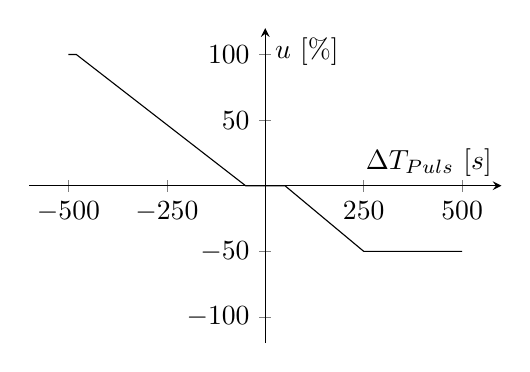
\begin{tikzpicture}
		\begin{axis}[%
				width=6cm,
				height=4cm,
				scale only axis,
				axis x line = center,
				axis y line = center,
				xlabel={$\Delta T_\mrm{Puls}$ $[\mrm{\upmu s}]$},
				ylabel={$u$ [\%]},
				xmin=-600, xmax=600,
				xtick={-500, -250, 0, 250, 500},
				ymin=-120, ymax=120,
				ytick={-100, -50, 0, 50, 100},
				legend pos = south east]

		\addplot [
				color=black,
				solid,
				forget plot
				]
			coordinates{
				(-500,100) (-480,100) (-50,0) (0,0) (50,0) (250,-50) (500,-50)
			};

		\end{axis}
	\end{tikzpicture}
	
	\caption{Kennlinie Fahrtenregler}%
	\label{fig:DrvCtrl:charact}%
\end{figure}

Aufgrund des eigentlichen Einsatzzweckes der Fahrtenregler weisen diese folgendes Verhalten auf:
\begin{itemize}
	\item Negative $\Delta T_\mrm{Puls}$, \dah kleinere Pulsbreiten als die Neutralstellung (außerhalb der Toleranzzone), führen immer zur Vorwärtsfahrt.
	\item Wenn von aus einer Vorwärtsbewegung zu positiven $\Delta T_\mrm{Puls}$ gewechselt wird, dann erfolgt eine Bremsung. Diese wird aber nicht über den Stillstand hinaus ausgeführt, \dah der Fahrtenregler stellt sicher, dass keine Rückwärtsbewegung eintritt.
	\item Um ausgehend von einer Vorwärtsfahrt Rückwärts zu fahren, muss der Fahrtenregler einmal mit positivem $\Delta T_\mrm{Puls}$ angesteuert werden (Bremsen), dann muss der Fahrtenregler mit einer Pulsbreite von \valunit{1,5}{ms} angesteuert werden. Damit ist die Rückwärtsfahrt "`freigeschaltet"'. Wenn jetzt wieder ein positives $\Delta T_\mrm{Puls}$ aufgebracht wird, dann erfolgt eine Rückwärtsfahrt. (Die Einzelschritte dieser Sequenz sind mindestens für \valunit{100}{ms} zu halten. Damit hat sich bisher immer eine sichere Umschaltung ergeben.)
\end{itemize}

Das ucboard bietet zur Ansteuerung zwei Möglichkeiten. Zum einen kann der Fahrtenregler "`direkt"' betrieben werden, \dah man dann den Wert für $\Delta T_\mrm{Puls}$ in Mikrosekunden direkt vorgeben. Die zweite Möglichkeit ist die der "`gemanagten"' Ansteuerung. Hierbei wird dem ucboard mitgeteilt, welche Fahrtrichtung gewählt werden soll und welche Stellgröße dabei verwendet werden soll. Dabei meint ein positiver Wert immer die gewählte Bewegungsrichtung, bei Vorwärtsfahrt bedeutet ein negativer Wert eine Bremsung. Dabei bildet bei Vorwärtsfahrt der Wertebereich von 1 bis 1\,000 den Stellgrößenbereich von 0 bis 100\,\% ab, bei Rückwärtsfahrt wird der Wertebereich von 1 bis 500 auf 0 bis $-50\,\%$ abgebildet. Ein Wert von 0 bedeutet Neutralstellung. Es ergeben sich damit die Kennlinien aus \figref{fig:DrvCtrl:charact_fb}.

\begin{figure}[htb]%
	\centering
	\subfloat[Vorwärts/Bremsen\label{fig:DrvCtrl:charact_f}]{%
		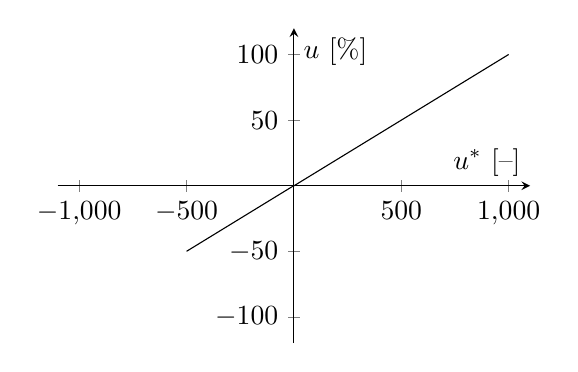
\begin{tikzpicture}
			\begin{axis}[%
					width=6cm,
					height=4cm,
					scale only axis,
					axis x line = center,
					axis y line = center,
					xlabel={$u^*$ [--]},
					ylabel={$u$ [\%]},
					xmin=-1100, xmax=1100,
					xtick={-1000, -500, 0, 500, 1000},
					ymin=-120, ymax=120,
					ytick={-100, -50, 0, 50, 100},
					legend pos = south east]

			\addplot [
					color=black,
					solid,
					forget plot
					]
				coordinates{
					(-500,-50) (-1,0) (0,0) (1,0) (1000,100)
				};

			\end{axis}
		\end{tikzpicture}
	}
	\hspace{2cm}
	\subfloat[Rückwärts\label{fig:DrvCtrl:charact_b}]{%
		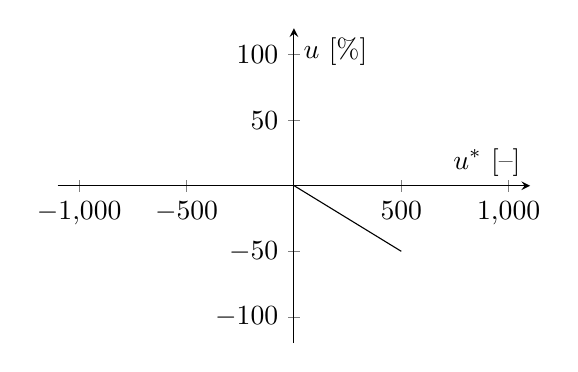
\begin{tikzpicture}
			\begin{axis}[%
					width=6cm,
					height=4cm,
					scale only axis,
					axis x line = center,
					axis y line = center,
					xlabel={$u^*$ [--]},
					ylabel={$u$ [\%]},
					xmin=-1100, xmax=1100,
					xtick={-1000, -500, 0, 500, 1000},
					ymin=-120, ymax=120,
					ytick={-100, -50, 0, 50, 100},
					legend pos = south east]

			\addplot [
					color=black,
					solid,
					forget plot
					]
				coordinates{
					(0,0) (1,0) (500,-50)
				};

			\end{axis}
		\end{tikzpicture}
	}
	\caption{Kennlinien zur "`gemanagten"' Ansteuerung über ucboard}%
	\label{fig:DrvCtrl:charact_fb}%
\end{figure}

Die für die Umschaltung von Vorwärts- auf Rückwärtsfahrt notwendige Bestimmung des Ist-Zustandes des Fahrtenreglers erfolgt dabei über einen Zustandsautomaten, der die Zustandswechsel des Fahrtenreglers nachbildet. Für den normalen Betrieb sollte dies sicher funktionieren. Fehler können nur dann auf"|treten, wenn
\begin{itemize}
	\item sehr schnell zwischen Vor- und Rückwärtsfahrt gewechselt wird (weniger als \valunit{200}{ms} zwischen aufeinanderfolgenden Wechsel) oder
	\item im Direktmodus Werte gestellt werden, die an den Rändern des Toleranzbereichs für die Neutralstellung liegen.
\end{itemize}
Erfolgt eine Vorwärtsfahrt (länger als \valunit{100}{ms}) stimmen die Zustände wieder überein.




Die Fahrtenregler sind hier so angeschlossen, dass \emph{keine} der \valunit{5}{V}-Spannungsversorgungsleitungen angeschlossen ist, sondern die Spannung direkt aus dem Fahrakku nimmt. Die Verbindung zum Fahrakku kann über das ucboard und den drvbatswitch geschaltet werden.



Die notwendige Massenverbindung als Bezug für das PWM-Signal wird über die Verbindung des ucboards mit dem drvbatswitch hergestellt. Dieses muss daher immer angeschlossen sein. (Ansonsten muss (nur!) die Masseleitung des nicht angeschlossenen Spannungsversorgungskabel des Fahrtenreglers an einen Massepin des ucboards angeschlossen werden.) 



\paragraph{Problemlösung}

\begin{itemize}
	\item Schalter des Fahrtenreglers am Chassis auf "`ON"'?
\end{itemize}



\section{Sensorik}

\subsection{Ultraschall}

Es sind drei Ultraschallsensoren des Typs SRF08 verbaut, jeweils einer nach vorne, nach links und nach rechts.

Es wird die Zeit $T_\mrm{echo}$ vom Aussenden des Ultraschallimpulses bis zum Empfang des ersten Echos gemessen.\footnote{Genau genommen werden auch noch möglicherweise auf"|tretende weitere Echos gemessen. Die dazugehörigen Zeiten stellt der Sensor in weiteren Registern zur Verfügung. Aktuell werden diese jedoch nicht ausgelesen. Möglicherweise könnte man mit einer Auswertung dieser Daten Fehlmessungen reduzieren.}

Der gemessene Abstand $d$ entspricht der halben Signallaufstrecke $c \cdot T_\mrm{echo}$, wobei für die Schallgeschwindigkeit $c = \valunit{343,2}{m/s}$ angenommmen wird. Es ergibt sich damit
\begin{align*}
	d = \frac{1}{2} \cdot c \cdot T_\mrm{echo} = \valunit{171,6}{\frac{m}{s}} \cdot T_\mrm{echo}\;.
\end{align*}


Der Sensor gibt die Zeiten $T_\mrm{echo}$ in Mikrosekunden zurück, wobei die Auf"|lösung \valunit{4}{\upmu s} ist. Damit ergibt sich eine Distanzauflösung von \ca \valunit{0,7}{mm}. Die Messwerte werden vom ucboard in \valunit{0,1}{mm} zurückgegeben.


\paragraph{Optionen: Messbereich und Verstärkung}

Siehe Datenblatt des Sensors.


\subsection{Hall-Sensor}

Mit dem Hall-Sensor (Typ HAL 503) kann die Drehzahl des hinteren linken Rades gemessen werden. Dazu sind auf der Felge des Rades über den Umfang acht Magnete verteilt, die von der Polarität her immer wechselweise angeordnet sind.

Der genannte Sensor besitzt zwei stabile Zustände. Wird ein positiver magnetischer Pol in die Nähe gebracht, so wechselt er in den Zustand 1, bei einem negativen magnetischen Pol in den Zustand 0. Liegt kein Feld vor, dann wird der alte Zustand gehalten. 

Somit kann durch Messen der Zeit zwischen zwei Zustandswechseln die Zeitdauer für eine achtel Umdrehung bestimmt werden. 

Auf dem ucboard wird die Zeit zwischen den Impulsen auf eine Mikrosekunde genau bestimmt. Die Ausgabe der Messwerte erfolgt dann in \valunit{0,1}{ms}. Daneben wird auch die Summe dieser Zeiten über acht Zustandswechsel, also einer Radumdrehung, bestimmt und in einer Genauigkeit von \valunit{1}{ms} ausgegeben. Zuletzt erfolgt auch die Ausgabe der Anzahl an gezählten Zustandswechseln in Modulo 256, wenn extern selber mitgezählt werden soll. (Letzteres erlaubt auch die Überprüfung, ob ggf. Messdaten verloren gegangen sind.)

Im Gegensatz zu einem "`klassischen"' Encoder kann die Drehrichtung nicht festgestellt werden!

\begin{itemize}
	\item Der Abstand zwischen Rad und Aufbau darf nicht zu groß sein. Ist das Fahrzeug beispielsweise aufgebockt, so werden in der Regel keine Impulse mehr gezählt.\footnote{Vom Hersteller gibt es noch einen Hall-Sensor aus der gleichen Baureihe (HAL 502), der jedoch etwas empfindlicher (die notwendige Flussdichte beträgt \ca ein Drittel im Vergleich zum HAL 503) ist. Sollten häufig Probleme mit übersprungenen Impulsen auf"|treten, wäre dies eine mögliche Lösung.}
\end{itemize}


\subsection{IMU}

Auf der hinteren rechten Ecke des ucboards befindet sich ein Beschleunigungs- und Drehratensensor (IMU -- Inertial Measurement Unit) des Typs MPU-9250A.

Die $x$-Achse zeigt nach vorne, die $y$-Achse nach links und die $z$-Achse nach oben.

Der Sensor gibt die Messwerte als \texttt{int16\_t}-Werte aus. Die Umrechnung eines Sensorwertes \texttt{val} in eine physikalische Einheit hängt von dem gewählten Messbereich ab. Für Beschleunigungswerte gilt
\begin{align}
	a(\mathtt{val})
		=
			\begin{cases}
				\frac{\mathtt{val}}{16\,384} g & \tn{wenn Messbereich } \pm 2\,g \\
				\frac{\mathtt{val}}{8\,192} g & \tn{wenn Messbereich } \pm 4\,g \\
				\frac{\mathtt{val}}{4\,096} g & \tn{wenn Messbereich } \pm 8\,g \\
				\frac{\mathtt{val}}{2\,048} g & \tn{wenn Messbereich } \pm 16\,g 
			\end{cases}
	\label{eq:hw:IMU:ACCScale}
\end{align}
und für Drehratenwerte gilt
\begin{align}
	\omega(\mathtt{val})
		=
			\begin{cases}
				\frac{\mathtt{val}}{131} \mrm{\degree / s} & \tn{wenn Messbereich } \pm \valunit{250}{\degree / s} \\
				\frac{\mathtt{val}}{65,5} \mrm{\degree / s} & \tn{wenn Messbereich } \pm \valunit{500}{\degree / s} \\
				\frac{\mathtt{val}}{32,8} \mrm{\degree / s} & \tn{wenn Messbereich } \pm \valunit{1000}{\degree / s} \\
				\frac{\mathtt{val}}{16,4} \mrm{\degree / s} & \tn{wenn Messbereich } \pm \valunit{2000}{\degree / s}\;.
			\end{cases}
	\label{eq:hw:IMU:GYROScale}
\end{align}

Standardmäßig sind die Messbereiche $\pm 4\,g$ und $\pm \valunit{500}{\degree / s}$ eingestellt. Diese können jedoch über entsprechende Befehle geändert werden.


\paragraph{Filterung}

Die IMU verfügt über digitale Filter, die vor der sensorinternen Unterabtastung angewendet werden. (Der genaue Aufbau der Filter ist nicht dokumentiert. Die Angabe über Bandbreite und Verzögerung ("`delay"') lassen aber darauf schließen, dass es sich im Wesentlichen um eine Mittelwertbildung handelt.) Die möglichen Einstellungen, die über die ucboard-Befehle vorgenommen werden können, sind in \tabref{tab:hw:imufilters} aufgeführt. Diese Werte sind den Einträgen in der "`Register Map"'-Dokumentation des MPU-9250 entnommen. 

\textbf{Hinweis:} Es ist zu beachten, dass die Abtastung (das Abfragen des Sensorwerte) seitens des ucboard unabhängig von der in \tabref{tab:hw:imufilters} \bzw im Sensordatenblatt genannten Abtastszeit immer mit \valunit{1}{kHz} erfolgt! Auch deshalb sollten die in \tabref{tab:hw:imufilters} grau geschriebenen Einstellungen nur zu Informationszwecken verwendet und nicht für den Normalbetrieb vorgesehen werden.

Die Standardeinstellung der Filter ist jeweils \verb|0|.

\begin{table}%
	\centering
	\caption{Filtereinstellungen IMU}
	\label{tab:hw:imufilters}
	\subfloat[Gyroskop \label{tab:hw:imufilters:gyro}]
	{%
		\begin{tabular}{cccc}
			\mytoprule
			\texttt{GFILT} & Bandbreite [Hz] & Verzögerung [ms] &  Interne Sensor- \\
			& & & abtastzeit [kHz] \\
			\mymidrule
			\color[rgb]{0.5,0.5,0.5}{\texttt{-2}} & \color[rgb]{0.5,0.5,0.5}{8\,800}   & \color[rgb]{0.5,0.5,0.5}{0,064} & \color[rgb]{0.5,0.5,0.5}{32}\\
			\color[rgb]{0.5,0.5,0.5}{\texttt{-1}} & \color[rgb]{0.5,0.5,0.5}{3\,600}   & \color[rgb]{0.5,0.5,0.5}{0,11} & \color[rgb]{0.5,0.5,0.5}{32} \\
			\texttt{0} & 250 & 0,97 & 8 \\
			\texttt{1} & 184 & 2,9 & 1 \\
			\texttt{2} & 92   & 3,9 & 1 \\
			\texttt{3} & 41  & 5,9 & 1 \\
			\texttt{4} & 20  & 9,9 & 1 \\
			\texttt{5} & 10  & 17,85 & 1 \\
			\texttt{6} & 5  & 33,38 & 1 \\
			\color[rgb]{0.5,0.5,0.5}{\texttt{7}} & \color[rgb]{0.5,0.5,0.5}{3\,600}  & \color[rgb]{0.5,0.5,0.5}{0,17} & \color[rgb]{0.5,0.5,0.5}{8} \\
			\mybottomrule
		\end{tabular}%
		}
	\\[10mm]
	\subfloat[Beschleunigungssensor \label{tab:hw:imufilters:acc}]
	{%
		\begin{tabular}{cccc}
			\mytoprule
			\texttt{AFILT} & Bandbreite [Hz] & Verzögerung [ms] &  Interne Sensor- \\
			& & & abtastzeit [kHz] \\
			\mymidrule
			\color[rgb]{0.5,0.5,0.5}{\texttt{-1}} & \color[rgb]{0.5,0.5,0.5}{1\,046} & \color[rgb]{0.5,0.5,0.5}{0,503} & \color[rgb]{0.5,0.5,0.5}{4} \\
			\texttt{0} & 218,1 & 1,88 & 1 \\
			\texttt{1} & 218,1 & 1,88 & 1 \\
			\texttt{2} & 99    & 2,88 & 1 \\
			\texttt{3} & 44,8  & 4,88 & 1 \\
			\texttt{4} & 21,2  & 8,87 & 1 \\
			\texttt{5} & 10,2  & 16,83 & 1 \\
			\texttt{6} & 5,05  & 32,48 & 1 \\
			\texttt{7} & 420   & 1,38 & 1 \\
			\mybottomrule
			\multicolumn{3}{p{8cm}}{\color[rgb]{1,0,0} \tiny Die Einstellungen \texttt{0} und \texttt{1} sind in der Dokumentation tatsächlich identisch angegeben. Das könnte man mal überprüfen.}
		\end{tabular}
		}
\end{table}



\subsection{Magnetometer}

Das Magnetometer vom Typ AK8963C ist im Gehäuse der IMU integriert. (Prinzipiell empfiehlt es sich, direkt das Datenblatt des AK8963 zu verwenden, und nicht in die entsprechenden Passagen des Datenblattes der IMU zu schauen.)

Die Achsenanordnung des Magnetometers unterscheidet sich von der der IMU \bzw damit auch der Achsenanordnung des Fahrzeugs. So zeigt die $x$-Achse zeigt nach links, die $y$-Achse nach vorne und die $z$-Achse nach unten. \textbf{\emph{Alle} ausgegebenen Werte werden jedoch in Fahrzeug- oder IMU-Koordinaten angegeben!}

Es liegt \ca alle \valunit{10}{ms} neue Messwerte vor. (Ungefähr, da die Taktrate des Mikrocontrollers und die des Sensors leicht abweichen können.)


\paragraph{Korrektur der Sensorempfindlichkeit}

Im Magnetometer ist intern für jede Achse ein Korrekturwert für die Sensitivität gespeichert (\texttt{ASAX}, \texttt{ASAY} und \texttt{ASAZ}). Dieser wird beim Starten ausgelesen und zur Korrektur der Messwerte verwendet. Diese Korrektur kann auch abgeschaltet werden (\verb|!MAG OPT ~USEASA=0|).

Der korrigierte Wert $H'_{\{\mrm{x,y,z}\}}$ ergibt sich aus dem Sensorwert $H_{\{\mrm{x,y,z}\}}$ und dem jeweiligen Korrekturfaktor \texttt{ASA}\{\texttt{X},\texttt{Y},\texttt{Z}\} über
\begin{align*}
	H'_{\{\mrm{x,y,z}\}} = H_{\{\mrm{x,y,z}\}} \cdot \left( \frac{(\mathtt{ASA}\{\mathtt{X},\mathtt{Y},\mathtt{Z}\} - 128) \cdot 0,5}{128} + 1 \right)\;.
\end{align*}


\paragraph{Kalibrierung des eingebauten Sensors}

Eine weitere Kalibrierung des Magnetometers ist für die Zukunft vorgesehen. Aktuell muss dies aber, wenn gewünscht \bzw notwendig, selber auf dem PC realisiert werden.


\paragraph{Berechnung des Kurswinkels}

Unter der Annahme, dass das Fahrzeug eben steht, kann aus dem Messwert der magnetischen Feldstärke in $x$- und $y$-Richtung der im(!) Uhrzeigersinn gezählte Kurswinkel $\psi_\mrm{h}$ über
\begin{align*}
	\psi_\mrm{h} = \mrm{atan2}(\mathtt{MY},\ \mathtt{MX})
\end{align*}
in Radiant bestimmt werden. Die Funktion atan2 gibt einen Wert zwischen $-\uppi$ und $\uppi$ zurück. Einen typischen "`Kompasswert"' in Grad erhält man daher nach dem Pseudocode
\begin{verbatimtab}[4]
	heading = atan2(MY, MX) * 180 / pi
	
	if heading < 0
		heading = 360 + heading
	end
\end{verbatimtab}



\section{Taster und LEDs}

Auf dem Board sind drei Taster (A, B und C) und zwei LEDs (A und B) vorhanden, die über die serielle Schnittstelle abgefragt \bzw gesetzt werden können. Für die LEDs SYS, DRVBAT und 12V ON ist keine externe Steuerung vorgesehen.


\paragraph{Abfrage Taster}

Die Abfrage der Tasterzustände erfolgt über die DAQ-Kanäle \verb|PBA|, \verb|PBB| und \verb|PBC|. Jeder dieser Kanäle gibt einen Zählerwert der Tasterbetätigungen zurück. Dieser Zähler wird für jedes Herunterdrücken und jedes Loslassen des Tasters inkrementiert. Ein betätigter Taster ist dabei durch eine gerade, und ein unbetätigter Taster durch eine ungerade Zahl repräsentiert. Auf diese Weise lassen sich auch sehr kurze Betätigungen erfassen, ohne dass die Abtastzeit des Kanals sehr klein eingestellt werden muss. Die Zähler sind Modulo 256.

\paragraph{LEDs}

Die LEDs können über einen entsprechenden Befehl ein- und ausgeschaltet werden. Auch können Blinksequenzen vorgegeben werden. Siehe dazu die Befehlsbeschreibung des Befehls \verb|LED|.


\FloatBarrier

\clearpage

\chapter{Kommunikation}


\section{Prinzip}

Die Kommunikation mit dem ucboard ist textbasiert, so dass eine Bedienung über ein einfaches Terminalprogramm möglich ist. Dies ermöglicht ein einfaches Testen und Debuggen. Um dennoch ein einfaches Parsen der Nachrichten zu ermöglichen, besitzen diese ein definiertes Format.

In der Regel sind alle Nachrichten auch einfach lesbar. Um bezüglich der Messdatenerfassung etwas platzeffizienter zu sein, können diese jedoch optional als hex- oder base64-codierte Binärdaten versendet werden.

Ebenso wird in der Regel auf Prüfsummen verzichtet. Lediglich bei Messdaten, die als Binärdaten verschickt werden, kann optional eine CRC16-Prüfsumme angehängt werden. (Bei manchen Befehlen zum ucboard besteht die Möglichkeit, die wesentliche Zahl doppelt zu senden.)

Messdaten und Textnachrichten können vom ucboard ohne Auf"|forderung versendet werden. Ansonsten reagiert das ucboard auf Befehle, die an dieses geschickt werden. Dabei wird jeder Befehl durch eine Antwort quitiert.

\begin{itemize}
	\item Die Nachrichten zum ucboard sollen sich möglichst einfach Parsen lassen. Die Nachrichten bestehen aus einem oder mehreren, durch Leerzeichen getrennte Wörter. Der Typ eines Wortes ergibt sich aus dem ersten Zeichen:
		\begin{itemize}
			\item \texttt{A} - \texttt{Z} und \texttt{\_}: String
			\item \verb+~+: Optionsname
			\item \texttt{0} - \texttt{9} und \texttt{-}: Zahl
		\end{itemize}
	\item Besteht eine Nachricht aus mehreren Wörtern, so spielt die Anzahl der Leerzeichen zwischen den Wörtern keine Rolle. (Mindestens eines!)
\end{itemize}

Prinzipiell wird nicht zwischen Groß- und Kleinschreibung unterschieden.

Ein Nachricht beginnt mit einem Startzeichen und endet mit einem Endezeichen. Das Startzeichen kann variieren. Bei Nachrichten zum ucboard ist dieses \texttt{!} oder \texttt{?}, bei Nachrichten vom ucboard \texttt{:}, \texttt{'} und \texttt{\#}. Nach dem Startzeichen kann, muss aber kein Leerzeichen folgen. Alle Startzeichen dürfen auch innerhalb der Nachrichten verwendet werden. Dort haben sie keine besondere Bedeutung. (Eine "`Aufsynchronisierung"' sollte also anhand des Endezeichens erfolgen.)

Das Endezeichen ist \texttt{\textbackslash n} (newline) bei Nachrichten zum ucboard und \texttt{\textbackslash 03} (ETX) bei Nachrichten vom ucboard. Die Motivation dahinter ist, dass damit bei Nachrichten zum ucboard eine einfaches Terminalprogramm verwendet werden kann, bei Nachrichten vom ucboard jedoch auch mehrzeiliger Text sinnvoll dargestellt werden kann.

Einzelne Zeilenumbrüche (leere Nachrichten) sind zu ignorieren. (Diese werden optional nach ETX vom ucboard verwendet, um die Darstellung im Terminprogramm zu verbessern.)


\subsubsection{Zu ucboard}
\begin{itemize}
	\item Befehle beginnen mit \texttt{!}
	\item Abfragen beginnen mit \texttt{?}
	\item Antworten auf Fragen des ucboard (im interaktiven Modus) besitzen keinen speziellen Beginn. (Sie dürfen aber auch mit \texttt{!} oder \texttt{?} beginnen.
	\item Das Ende einer Nachricht wird ausschließlich durch \texttt{\textbackslash n} (newline) markiert
	\item Optionen beginnen mit \verb+~+. Wenn der Option ein Wert zugeordnet wird, dann wird dieser nach einem \texttt{=} angeschlossen. Dabei dürfen um das Gleichheitszeichen herum keine Leerzeichen stehen!
	\item Die Reihenfolge der Argumente spielt eine Rolle. Die Position der Optionen spielt keine Rolle. (Bei Verarbeiten im ucboard wird zunächst eine Liste der Argumente und eine Liste der Optionen erstellt. Die Information, ob eine Option am Anfang, zwischen zwei Argumenten oder am Ende stand geht dabei verloren.)
\end{itemize}


\subsubsection{Von ucboard}
\begin{itemize}
	\item Direkte Antworten beginnen mit \texttt{:}
	\item Auch jeder Schreibbefehl sollte eine kurze Antwort zur Quittierung senden, \zB \verb+:ok\n+. Es wäre empfehlenswert, den gesetzten Wert zu wiederholen
	\item Fehler bei der Abarbeitung von Befehlen beginnen mit \texttt{:ERR(code)}, wobei \texttt{code} eine positive Ganzzahl als Fehlercode ist. Optional kann nach einem weiteren Doppelpunkt eine Beschreibung des Fehlers folgen: \texttt{:ERR(code):Beschreibung} 
	\item Textausgaben (Display-Funktion) beginnen mit \texttt{'}
	\item Fehlermeldungen sind Textausgaben. Diese beginnen mit \texttt{'ERR(code)}, wobei \texttt{code} eine positive Ganzzahl als Fehlercode ist. Optional kann nach einem weiteren Doppelpunkt eine Beschreibung des Fehlers folgen: \texttt{'ERR(code):Beschreibung} 
	\item Ohne Auf"|forderung versendete Messdaten beginnen mit \texttt{\#} (base64- oder hex-codiert) \bzw \texttt{\#\#} (lesbarer Text).
	\item Wenn eine Nutzerinteraktion notwendig ist, dann sollte das letzte Zeichen vor dem Nachrichtendezeichen ein \texttt{?} oder \texttt{:} sein.
	\item Alle Nachrichten vom ucboard haben ETX (0x03) als Endzeichen. (Dadurch ist es möglich, eine mehrzeilige Ausgabe auf dem Terminalprogramm zu erzeugen.)
		\begin{itemize}
			\item Über eine -- aktuell noch fest eingestellte Option -- wird nach jedem ETX automatisch ein Zeilenumbruch geschickt. Dies dient der besseren Lesbarkeit. Es wäre jedoch besser, ein Terminalprogramm zu verwenden (\bzw zu schreiben), welches ETX durch einen Zeilenumbruch ersetzt. Damit wäre sowohl der Text besser lesbar als auch der Sparsamkeit Rechnung getragen.
			%\item Für die bessere Lesbarkeit ist es empfehlenswert, alle Textnachrichten mit einem Zeilenumbruch (vor ETX) abzuschließen. Lediglich bei hex- oder base64-basierten Messdatennachrichten wird dies nicht gemacht, da diese gerade für eine sparsame Kommunikation gedacht sind.
		\end{itemize}
\end{itemize}



\section{Hardware}

Das ucboard verfügt über zwei Schnittstellen für die Kommunikation mit dem PC. Zum einen kann über einen USB-Anschluss eine serielle Kommunikation aufgebaut werden und zum anderen kann eine RS232-Schnittstelle verwendet werden. Die RS232-Schnittstelle wird dabei nicht als Standard-D-SUB-Stecker (9-polig) angeboten, sondern als Wannensteckeranschluss. Dieser ist so belegt, dass eine direkte Verbindung zu den Anschlüssen des Onboard-PC über ein Flachbandkabel erfolgen kann.

Der dritte, "`reine"' UART-Anschluss ist für den Anschluss möglicher Erweiterungen und nicht die Kommunikation mit dem PC vorgesehen.\footnote{Man könnte auch noch darüber nachdenken, die dritte UART auch für die Kommunikation mit einem PC zu verwenden, da an dieser einfach ein Bluetooth-Adapter angeschlossen werden könnte. Damit wäre es möglich, auch ohne den Onboard-PC das Fahrzeug ferngesteuert zu betreiben.}


Die Parameter der Schnittstellen sind in \tabref{tab:Comm:UARTParam} zusammengefasst.

\begin{table}%
	\centering
	\caption{Einstellungen serielle Schnittstellen}
	\label{tab:Comm:UARTParam}
	\begin{tabular}{lcr}
			\mytoprule
			 & USB & RS232 \\
			\mymidrule
			Baudrate & 921\,600 & 115\,200 \\
			Datenbits & 8 & 8 \\
			Stopbits & 1 & 1 \\
			Parity & keine & keine \\
			Hardware-Flowcontrol & Nein & Nein \\
			\mybottomrule
	\end{tabular}\\
	\color[rgb]{1,0,0}{ToDo: Testen, welche Baudrate jeweils maximal möglich ist!} \textcolor[rgb]{0.75,0.75,0.75}{\footnotesize{Man könnte dies auch über einen Befehl einstellbar machen, und ein Rücksetzen darüber erreichen, dass beim Starten des ucboards \zB der Taster A betätigt wird. Aber das erscheint mir für diesen Zweck unnötig.}}
\end{table}


\section{Befehle}

\subsection{Übersicht}

\begin{table}[htbp]%
	\centering
	\caption{Übersicht über Hauptbefehle ucboard}
	\label{tab:Comm:Cmds}
	\begin{tabular}{ll}
		\mytoprule
		\verb|RESET| & Neustart ucboard \\
		\verb|VER| & Abfrage Softwareversion \\
		\verb|ID|	& Abfragen der Fahrzeug-ID \\
		\verb|SID| & Setzen und Abfragen der Session-ID \\
		\verb|TICS| & Abfrage ucboard-Zeit (Millisekunden nach (Neu)start) \\
		\verb|STEER| & Setzen und Abfragen des (Soll-)Lenkwinkels \\
		\verb|DRV| & Setzen und Abfragen der Fahrgeschwindigkeit \\
		\verb|DAQ| & Datenerfassung \\
		\verb|VOUT| & Ein- und Ausschalten \valunit{12}{V}-Ausgang (Kinect) \\
		\texttt{IMU} & Zum Parametrieren der IMU \\
		\texttt{MAG} & Zum Parametrieren des Magnetometers \\
		\texttt{US} & Zum Parametrieren der US-Sensoren \\
		\textcolor[rgb]{0.75,0.75,0.75}{\texttt{EEPROM}} & \textcolor[rgb]{0.75,0.75,0.75}{Zum Auslesen des EEPROM-Inhalts}\\
		\verb|LED| & Ansteuerung der LEDs A und B auf dem Board \\
		\mybottomrule
	\end{tabular}
\end{table}



\textbf{Wichtig:} Momentan werden numerische Eingaben noch nicht an allen Stellen daraufhin überprüft, ob es tatsächlich eine (Ganz)Zahl ist. Dies bedeutet, dass \zB Eingaben wie \verb|1000.|, \verb|1000.0| oder auch \verb|+1000| für Tausend eine unerwartete Zahl ergibt.


\subsection{Beschreibung}

\subsubsection{RESET}

Führt einen Neustart des ucboards durch.


\begin{verbatim}
	!RESET NOW
\end{verbatim}



\subsubsection{VER}

Fragt Versionsstring der ucboard-Software ab.


\begin{verbatim}
	?VER
	:0.1.x
\end{verbatim}



\subsubsection{ID}

Zur Abfrage der Fahrzeug-ID, also der Nummer, die über die Dipschalter auf der Platine eingestellt wird.


\begin{verbatim}
	?ID
	:4
\end{verbatim}


\subsubsection{SID}

Zum Abfragen und Setzen der Session-ID. Dies ist einfach eine Zahl, die nach einem Neustart des ucboards auf 0 gesetzt wird, und der beliebige \verb|uint32|-Werte gegeben werden können.


\begin{verbatim}
	?SID
	:0
\end{verbatim}

\begin{verbatim}
	!SID 25363
	:25363
\end{verbatim}

\begin{verbatim}
	?SID
	:25363
\end{verbatim}




\subsubsection{STEER}

Zum Setzen und Abfragen des Soll-Lenkwinkels (Servo-Vorgabe). Der Wert muss eine Ganzzahl zwischen $-1\,000$ und $1\,000$ sein.

Setzen:
\begin{verbatim}
	!STEER -200
	:-200
\end{verbatim}

Optionale Wiederholung des Arguments, um Fehlübertragungen zu detektieren:
\begin{verbatim}
	!STEER -200 -200
	:-200
\end{verbatim}

\begin{verbatim}
	!STEER -200 -201
	:ERR(269): Message corrupted! (The two values have to be equal!)
\end{verbatim}



Abfragen:
\begin{verbatim}
	?STEER
	:-200
\end{verbatim}



\subsubsection{DRV}

Zum Setzen und Abfragen der Fahrgeschwindigkeit. (\Bzw Motorspannung.)

Es gibt zwei Modi: Die "`gemanagte"' und die "`direkte"' Ansteuerung. Siehe dazu \secref{sec:hw:drivectrl}.


\paragraph{Gemanagte Ansteuerung}

Bei der gemanagten Ansteuerung erfolgt die Umschaltung von Vorwärts- und Rückwärtsfahrt automatisch. Zudem wird der gesetzte Wert in den Arbeitsbereich umgerechnet.

Vorwärtsfahrt:
\begin{verbatim}
	!DRV F 300
	:F 300
\end{verbatim}
Optionale Wiederholung des Arguments, um Fehlübertragungen zu detektieren:
\begin{verbatim}
	!DRV F 300 300
	:F 300
\end{verbatim}

\begin{verbatim}
	!drv f 300 301
	:ERR(269): Message corrupted! (The two values have to be equal!)
\end{verbatim}


Es sind Werte von -500 bis 1000 zulässig. Dabei entsprechen negative Werte Bremsen (aber nicht einer Rückwärtsfahrt!).

Die effektive Auf"|lösung ist geringer als der Stellbereich von 1000 es annehmen lässt. Tatsächlich können etwas weniger als 450 unterscheidbare Impulsbreiten, \dah Sollwerte, vorgegeben werden.

Bremsen
\begin{verbatim}
	!DRV F -500
	:F -500
\end{verbatim}
Gebremst wird vom Fahrtenregler automatisch nur bis zum Stillstand. Es erfolgt keine Rückwärtsfahrt.


Rückwärtsfahrt
\begin{verbatim}
	!DRV B 300
	:B 300
\end{verbatim}
Es sind Werte von 0 bis 500 zulässig. (Der Stellbereich des Fahrtenreglers ist rückwärts nur halb so groß wie vorwärts.)




Ausschalten des Fahrtenreglers:
\begin{verbatim}
	!DRV OFF
	:OFF
\end{verbatim}
Der Unterschied zwischen den Werten 0 und \verb|OFF| liegt darin, dass bei \verb|OFF| der Fahrtenregler vom Fahrakku getrennt wird, also tatsächlich ausgeschaltet ist. Der Fahrtenregler wird bei Übermittlung des nächsten Sollwertes ungleich \verb|OFF| automatisch wieder eingeschaltet, jedoch dauert dies einen Moment. (Das Einschalten wird auch mit einem Piepston des Fahrtenreglers begleitet.)


Abfragen:
\begin{verbatim}
	?DRV
	:F 300
\end{verbatim}


Abfragen der tatsächlichen Impulsbreite (vergleiche "`Direkte Ansteuerung"'):
\begin{verbatim}
	?DRV D
	:D -186
\end{verbatim}


\paragraph{Direkte Ansteuerung}
Bei der direkten Ansteuerung wird direkt die Impulsbreite vorgegeben, die an den Fahrtenregler übertragen wird. Dabei wird die Impulsbreite als die Abweichung in Mikrosekunden vom Neutralwert \valunit{1,5}{ms} angegeben. \Dah ein Wert von $-500$ entspricht der minimalen Impulsbreite (\dah Maximalwert \emph{vorwärts}) von \valunit{1}{ms} und ein Wert von 500 der maximalen Impulsbreite von \valunit{2}{ms}.


\begin{verbatim}
	!DRV D 200
	:D 200
\end{verbatim}





\paragraph{DMS}

Die Totmannschaltung (DMS -- Dead-man switch) soll insbesondere im Entwicklungsstatus der PC-Software und der Algorithmen verhindern, dass das Fahrzeug bei abgestürztem PC oder abgestürzten ROS-Nodes weiterfährt.

Dieser Parameter gibt die Zeit in Millisekunden an, innerhalb derer eine neue DRV-Nachricht erhalten sein muss. Wird diese Zeit ohne DRV-Nachricht überschritten, so wird der Motor gestoppt, \dah der Sollwert auf 0 (aber nicht \texttt{OFF}) gesetzt. Bei der nächsten \texttt{DRV}-Nachricht wird der Motor dann wieder angesteuert.

\begin{verbatim}
	!DRV ~DMS=1000
	:~DMS=1000
\end{verbatim}
Zum Abschalten der Sicherheitsschaltung dient der Wert \texttt{0}.

DRV kann auch ohne Parameter aufgerufen werden. Dann dient er nur dazu, die Zeitzählung der Totmannschaltung neu zu starten.

\begin{verbatim}
	!DRV
	:ok
\end{verbatim}

Abfrage der DMS-Abschaltzeit zusammen mit dem aktuellen DRV-Wert:
\begin{verbatim}
	?DRV ~DMS
	:OFF ~DMS=1000
\end{verbatim}



\subsubsection{DAQ}

Das Datenerfassungsmodul (DAQ -- Data Aquisition) dient als allgemeine Schnittstelle zur Übermittlung aller Sensorsignale. Dabei können Einzelabfragen vorgenommen werden (die angefragten Sensorwerte werden direkt als Antwort auf einen entsprechenden Befehl verschickt) als auch Gruppen von Sensorsignale eingerichtet werden, die dann automatisch vom ucboard an den PC geschickt werden.

Die Sensorsignale werden dabei hier als "`Kanäle"' bezeichnet. Die aktuell definierten Kanäle sind in \tabref{tab:Comm:DAQ:Signals} zusammengefasst.

\begin{table}[htbp]%
	\centering
	\caption{DAQ-Kanäle (Signale)}
	\label{tab:Comm:DAQ:Signals}
	\begin{tabular}{lp{8cm}lll}
		\mytoprule
		Kanal & Beschreibung & Einheit & Datentyp & Länge \\
		\mymidrule
		\verb|AX| & Beschleunigung $x$-Richtung & $\to$ \eqref{eq:hw:IMU:ACCScale} & \verb|int16_t| & 2 \\
		\verb|AY| & Beschleunigung $y$-Richtung & $\to$ \eqref{eq:hw:IMU:ACCScale} & \verb|int16_t| & 2 \\
		\verb|AZ| & Beschleunigung $z$-Richtung & $\to$ \eqref{eq:hw:IMU:ACCScale} & \verb|int16_t| & 2 \\
		\verb|GX| & Drehrate um $x$-Achse & $\to$ \eqref{eq:hw:IMU:GYROScale} & \verb|int16_t| & 2 \\
		\verb|GY| & Drehrate um $y$-Achse & $\to$ \eqref{eq:hw:IMU:GYROScale} & \verb|int16_t| & 2 \\
		\verb|GZ| & Drehrate um $z$-Achse & $\to$ \eqref{eq:hw:IMU:GYROScale} & \verb|int16_t| & 2 \\
		\verb|MX| & Magnetische Flussdichte in $x$-Achse & \valunit{0,15}{\upmu T} & \verb|int16_t| & 2\\
		\verb|MY| & Magnetische Flussdichte in $y$-Achse & \valunit{0,15}{\upmu T}  & \verb|int16_t| & 2\\
		\verb|MZ| & Magnetische Flussdichte in $z$-Achse & \valunit{0,15}{\upmu T}  & \verb|int16_t| & 2\\
		\verb|USF| & Abstand vorne & \valunit{0,1}{mm} & \verb|uint16_t| & 2 \\
		\verb|USL| & Abstand links & \valunit{0,1}{mm} & \verb|uint16_t| & 2 \\
		\verb|USR| & Abstand rechts & \valunit{0,1}{mm} & \verb|uint16_t| & 2 \\
		\verb|VSBAT| & Spannung Systemakku & mV & \verb|uint16_t| & 2\\
		\verb|VDBAT| & Spannung Fahrakku & mV & \verb|uint16_t| & 2\\
		\verb|HALL_DT| & Zeit zwischen den letzten beiden Impulsen des Hallsensors (eine Achtel Radumdrehung) & \valunit{0,1}{ms} & \verb|uint16_t| & 2\\
		\verb|HALL_DT8| & Zeit zwischen den letzten acht Impulsen des Hallsensors (eine Radumdrehung) & \valunit{1}{ms} & \verb|uint16_t| & 2\\
		\verb|HALL_CNT| & Anzahl der Sensorimpulse, Modulo 256 (Ein Sensorwert von "`1"' entspricht dabei immer eine ungeraden Zahl) & -- & \verb|uint8_t| & 1\\
		\verb|PBA| & Zähler Betätigung Taster A, Modulo 256 (Gerade Werte: Unbetätigt, Ungerade Werte: Betätigt)  & -- & \verb|uint8_t| & 1\\
		\verb|PBB| & wie \verb|PBA| für Taster B & -- & \verb|uint8_t| & 1\\
		\verb|PBC| & wie \verb|PBA| für Taster C & -- & \verb|uint8_t| & 1\\
		\mybottomrule
	\end{tabular}
\end{table}


Zur Übermittlung von Fehlerwerten sind bestimmte Zahlenwerte oder Textausgaben vorgesehen, die in \tabref{tab:Comm:DAQ:SpecialValues} aufgeführt sind. Dabei ist "`keine Daten vorhanden"' ein Wert, der vom DAQ-Modul selber gesetzt werden, wenn keine gültigen Daten vorliegen. Die einzelnen Sensormodule geben im Fehlerfall entweder "`Messfehler"' (bei einzelnen Messfehlern oder Messaussetzern) oder "`Sensorfehler"' (ein größeres Sensorproblem, \dah es ist in diesem Fall mit dem Ausfall aller (weiteren) Messwerten zu rechnen) zurück.


\begin{table}[htbp]%
	\centering
	\caption{Fehlerwerte}
	\label{tab:Comm:DAQ:SpecialValues}
	\subfloat[Binärcodierung]{%
		\begin{tabular}{lcccccc}
			\mytoprule
			Datentyp & \texttt{uint32\_t} & \texttt{int32\_t} & \texttt{uint16\_t} & \texttt{int16\_t} & \texttt{uint8\_t} & \texttt{int8\_t} \\
			\mymidrule
			Keine Daten vorhanden & \texttt{0xFFFFFFFF} & \texttt{0x7FFFFFFF} & \texttt{0xFFFF} & \texttt{0x7FFF} & \texttt{0xFF} & \texttt{0x7F} \\
			Messfehler & \texttt{0xFFFFFFFE} & \texttt{0x7FFFFFFE} & \texttt{0xFFFE} & \texttt{0x7FFE} & \texttt{0xFE} & \texttt{0x7E} \\
			Sensorfehler & \texttt{0xFFFFFFFD} & \texttt{0x7FFFFFFD} & \texttt{0xFFFD} & \texttt{0x7FFD} & \texttt{0xFD} & \texttt{0x7D} \\
			Wert zu groß oder zu klein  & \texttt{0xFFFFFFFC} & \texttt{0x7FFFFFFC} & \texttt{0xFFFC} & \texttt{0x7FFC} & \texttt{0xFC} & \texttt{0x7C} \\
			Wert zu groß  & \texttt{0xFFFFFFFC} & \texttt{0x7FFFFFFC} & \texttt{0xFFFC} & \texttt{0x7FFC} & \texttt{0xFC} & \texttt{0x7C} \\
			Wert zu klein & \texttt{0xFFFFFFFB} & \texttt{0x7FFFFFFB} & \texttt{0xFFFB} & \texttt{0x7FFB} & \texttt{0xFB} & \texttt{0x7B} \\
			\mybottomrule
		\end{tabular}}\\
	\subfloat[Textausgabe]{%
		\begin{tabular}{lc}
			\mytoprule
			 & \\
			\mymidrule
			Keine Daten vorhanden & \texttt{[-{}-{}-]}  \\
			Messfehler & \texttt{[mfault]}  \\
			Sensorfehler & \texttt{[fault]} \\
			Wert zu groß oder zu klein & \texttt{[range]} \\
			Wert zu groß  & \texttt{[over]}  \\
			Wert zu klein & \texttt{[under]} \\
			\mybottomrule
		\end{tabular}}
\end{table}



\paragraph{Allgemeines}

Alle aktuell definierten Kanäle können mit \verb|?DAQ CHS| abgefragt werden:
\begin{verbatim}
	?DAQ CHS
	:14
	AX         | acc. ahead                     | opt-dep.!       | 1     | I16 
	AY         | acc. left                      | opt-dep.!       | 1     | I16 
	[...]
	HALL_DT8   | delta time full rev.           | 1 ms            | undef | U16 
\end{verbatim}
Dabei beinhalten die Spalten die folgenden Informationen
\begin{itemize}
	\item Name
	\item Beschreibung
	\item Einheit (\verb|opt-dep.!| bedeutet, dass die Einheit von den jeweiligen Sensoreinstellungen abhängt.)
	\item Abtastzeit in Millisekunden (\verb|undef| bedeutet, dass das entsprechende Sensormodul keine feste Abtastzeit der Messwerte garantiert.)
	\item Datentyp
\end{itemize}

Die Informationen zu einem speziellen Kanal können über
\begin{verbatim}
	?DAQ CH name
\end{verbatim}
abgefragt werden:
\begin{verbatim}
	?DAQ CH USF
	:USF        | ultrasonic front distance      | 0.1 mm          | undef | U16
\end{verbatim}



\paragraph{Einzelabfrage von Werten}

Zur Abfrage von Einzelwerten dient der Subbefehl \verb|GET|:
\begin{verbatim}
	?DAQ GET chname1 [chname2 [chname3 [...]]] [~AGE] [~TICS]
\end{verbatim}
Diesem muss mindestens der Name eines Kanals übergeben werden. Es können aber auch mehrere Kanäle auf einmal abgefragt werden. Die Option \verb|~AGE| gibt zu \emph{jedem} Wert das Alter in Tics (\dah ms) zwischen dem Zeitpunkt der Datenerfassung und der Datenabfrage zurück. Die Option \verb|~TICS| gibt zu \emph{jedem} Wert den Erfassungszeitpunkt in Tics zurück. Sind beide Optionen gewählt, dann wird immer AGE vor TICS zurückgegeben, unabhängig von der Reihenfolge der Optionen.

Beispiele:

\begin{itemize}
	\item Einzelabfrage des Sensorwertes des vorderen Ultraschallsensors
		\begin{verbatim}
			?DAQ GET USF
			:1860
		\end{verbatim}
	\item Ausgabe des Alters des Messwertes
		\begin{verbatim}
			?DAQ GET ~AGE USF
			:1860 68
		\end{verbatim}
	\item Abfrage aller Ultraschallwerte, jeweils mit Alter
		\begin{verbatim}
			?DAQ GET ~AGE USL USF USR
			:487 72 | 1860 75 | 4293 85
		\end{verbatim}
	\item Ausgabe der ucboard-Zeit des Messwerts
		\begin{verbatim}
			?DAQ GET ~TICS USF
			:1860 3059246
		\end{verbatim}
\end{itemize}
















\paragraph{Automatische Messgruppen}

Es stehen zwanzig parametrierbare Messgruppen zur Verfügung, die zum automatischen Verschicken von Messdaten verwendet werden. In diesen können bis zu zehn verschiedene Kanäle (Sensorwerte) zusammengefasst werden. Neben den normalen Kanälen stehen noch die in \tabref{tab:Comm:DAQ:SpecialChannels} aufgeführten "`Sonderkanäle"' zur Verfügung, die Metadaten zu den Datensätzen enthalten. (Diese stehen bei der Einzelabfrage über \verb|?DAQ GET chname| nicht zur Verfügung.)

Es wird je Gruppe immer nur ein Messdatensatz gepuffert. Kann dieser nicht verschickt werden, bis die nächste Abtastung der Gruppe erfolgt ist, so wird dieser verworfen. Dabei werden alle Gruppen gleichberechtigt behandelt, \dah es erfolgt keine Bevorzugung von Messgruppen mit kleiner Abtastzeit. Damit ist die Wahrscheinlichkeit gering, dass bei langsam abgetasteten Messgruppen Daten verlorengehen, auch wenn viel Bandbreite für Messgruppen mit kleiner Abtastzeit belegt wird.\footnote{An dieser Stelle muss noch angemerkt werden, dass das Management der zu versendenden Daten im Idle-Task des ucboards erfolgt. \Dah während der Datenerfassung im SysTick-Task werden keine neuen Daten zum Verschicken bereit gemacht, auch wenn der letzte Datensatz abgearbeitet ist. Damit ist der erreichbare Datendurchsatz kleiner als der sich theoretisch aus der Baudrate ergebenden Wert. Dies kann \bzw sollte in Zukunft noch geändert werden. Bisher benötigt der SysTick-Task weniger als \valunit{200}{\upmu s}. Damit würde im ungünstigsten Fall die Datenrate ein Fünftel "`verlieren"'.}

Eine Messgruppe wird über den Subbefehl \verb|GRP| definiert.
\begin{verbatim}
	!DAQ GRP grpnb chname1 [chname2 [chname3 [...]]] [~option1] [~option2] [...]
\end{verbatim}
Die Gruppennummer \verb|grpnb| muss eine Ganzzahl zwischen 0 und 19 sein.

Die Möglichkeiten der Gruppendefinition wird zunächst an Beispielen demonstriert. Danach werden die Optionen genauer beschrieben.
\begin{itemize}
	\item Gruppe 1 enthält die Werte des Ultraschalls. Es wird gesendet, wenn alle Ultraschallwerte vorliegen, wobei maximal \valunit{10}{ms} nach dem Erfassen des ersten Wertes gewartet wird. Die Daten werden base64-codiert und mit einer CRC16-Prüfsumme verschickt.
		\begin{verbatim}
			!DAQ GRP 1 ~ALL=10 ~ENC=B64 ~CRC _TIC USL USF USR 
		\end{verbatim}
		(Die Reihenfolge der Kanalnamen (\verb|_TIC|, \verb|USL|, \verb|USF|, \verb|USR|) spielt eine Rolle, da die Messwerte ohne Namen in dieser Reihenfolge ausgegeben werden. Die Reihenfolge der Optionen und ob diese am Anfang oder Ende oder auch zwischen den Kanalnamen stehen spielt keine Rolle.)
	\item Gruppe 2 enthält die Spannungen der beiden Akkus, wobei immer eine Nachricht verschickt wird, sobald eine neue Spannung gemessen ist.
		\begin{verbatim}
			!DAQ GRP 2 ~ANY VSBAT VDBAT 
		\end{verbatim}
	\item Gruppe 3 enthält die Beschleunigungswerte in der Ebene und die Gierrate. Die Daten werden alle \valunit{10}{ms} verschickt. Dabei werden alle innerhalb der \valunit{10}{ms} erfassten Daten gemittelt.
		\begin{verbatim}
			!DAQ GRP 3 ~TS=10 ~AVG ~ENC=B64 ~CRC AX AY GZ 
		\end{verbatim}
\end{itemize}


Optionen:
\begin{itemize}
	\item Modus Abtastung
		\begin{itemize}
			\item \verb+~ALL[=maxwait]+: Sendet, wenn zu allen Gruppenkanäle neue Daten vorhanden sind. Wenn \verb+maxwait+ gegeben ist, dann wird nach dem ersten neuen Wert maximal diese Zeit in Millisekunden gewartet, bis die Daten verschickt werden.\footnote{Dies ist \zB für die US-Sensoren gedacht, deren Daten meist an nacheinander liegenden Zeitschritten ankommen.}
			\item \verb+~ANY+: Sendet, wenn zu einem der Gruppenkanäle ein neues Datum vorhanden ist.
			\item \verb+~TS=Ts+: Abtastzeit in Millisekunden. (Muss ein ganzes Vielfaches der Abtastzeiten aller Kanäle des Paketes sein.)
			\begin{itemize}
				\item \verb+~AVG[=Ta]+: Mittelung über Zeitraum \verb|Ta|. (Nur im Abtastmodus \verb|TS| verfügbar.) Wenn die Option \verb|AVG| verwendet wird, dann müssen alle Gruppenkanäle die gleiche Abtastzeit besitzen. \verb|Ta| darf dabei maximal \verb|Ts| sein und muss ein ganzes Vielfaches der Abtastzeit der Gruppenkanäle sein. Wenn kein \verb|Ta| angegeben ist, dann wird \verb|Ta| = \verb|Ts| gesetzt.\\
				Diese Mittelung kann damit bezüglich der Sensorabtastzeit $T_\mrm{s,sig}$ über die Übertragungsfunktion
				\begin{align*}
					G_\mrm{avg}(z) = \frac{\frac{1}{n_\mrm{avg}} \cdot ( z^{n_\mrm{avg}-1} + z^{n_\mrm{avg}-2} + \cdots + 1)}{z^{n_\mrm{avg}-1}}
				\end{align*}
				mit $n_\mrm{avg} = \mathtt{Ta}/T_\mrm{s,sig}$ ausgedrückt werden. Über \verb+~TS=Ts+ wird dann eine Unterabtastung mit dem Faktor $\mathtt{Ts}/T_\mrm{s,sig}$ vorgenommen.
			\end{itemize}
			
				
		\end{itemize}
	\item \verb+~SKIP=n+: Überspringt \texttt{n} Werte. \Dah bei einem Wert von neun wird jeder zehnte Wert verwendet. Dieses Überspringen wird nach allen anderen Berechnungen und Abfragen durchgeführt. Diese Option dient primär zum Debuggen (um die Menge an ausgegebenem Text zu reduzieren), kann aber auch zur Unterabtastung für Kanäle ohne feste Abtastzeit verwendet werden. (Dabei ist dann aber keine Mittelung möglich.)
	\item \verb+~ENC=B64|HEX|ASCII+: Nachricht wird base64-codiert (ohne Padding), Hex-codiert oder Ascii-codiert. ASCII meint hierbei "`lesbaren Text"'. Standardwert ist ASCII.
	\item \verb+~CRC+: CRC16-Prüfsumme (Nur wenn ENC = B64 oder HEX)\\
		Berechnung mit:
		\begin{lstlisting}[style=C_colored_smallfont]
// from Antonio Pires, http://stackoverflow.com/questions/10564491/function-to-calculate-a-crc16-checksum

// CRC-16-CCITT (polynom 0x1021)


uint16_t crc16(uint8_t* data_p, uint16_t length)
{
	uint8_t x;
	uint16_t crc = 0xFFFF;

    while (length--)
    {
        x = (crc >> 8) ^ (*data_p++);
        x ^= (x >> 4);
        crc = (crc << 8) ^ ((uint16_t)(x << 12)) ^ ((uint16_t)(x <<5)) ^ ((uint16_t)x);
    }

    return crc;
}
		\end{lstlisting}
	\item \verb+~AGE+ und \verb+~TICS+: Wie bei Einzelwertabfrage. Damit wird \emph{jedem} Wert das Alter sowie der Erfassungszeitpunkt hinzugefügt. (Wenn beide Optionen gewählt sind, dann immer in der Reihenfolge "`Age -- Tics"'.) Die Werte werden bei der Ascii-Codierung immer innerhalb der senkrechten Striche des Kanals geschrieben. Bei Binärcodierungen werden diese Werte jeweils als \valunit{32}{bit}-Werte jeweils hinter den betreffenden Messwert eingefügt. Diese Optionen dienen lediglich zum Debuggen. Im "`Normalbetrieb"' sollten diese aufgrund des großen Platzbedarfs nicht verwendet werden!\footnote{Das Alter \texttt{AGE} bezieht sich auf den Abtastzeitpunkt des Datensatzes, nicht auf den Zeitpunkt des Versendens. Der Wert ist damit nur bei der Abtastart \texttt{ALL} relevant, da dort die Daten einer Gruppe zu unterschiedlichen Zeitpunkten abgetastet sein können. Die Zeitdifferenz zwischen Abtastzeitpunkt und Versenden kann durch den Sonderkanal \texttt{\_DLY} abgefragt werden. (Somit ist das tatsächliche Alter \texttt{AGE} + \texttt{\_DLY} plus die Zeit zur Datenübermittlung und Verzögerungen innerhalb des Betriebssystem des PCs.)}
\end{itemize}


\begin{table}[htbp]%
	\centering
	\caption{"`Sonderkanäle"' mit Metadaten}
	\label{tab:Comm:DAQ:SpecialChannels}
	\begin{tabular}{lp{10cm}lll}
		\mytoprule
		Signal & Beschreibung & & Datentyp & Länge \\
		\mymidrule
		\verb|_CNT| & Anzahl der verschickten Datensätze der Gruppe &  & \verb|uint32_t| & 4 \\
		\verb|_CNT16| & die niederwertigen \valunit{16}{bits} von \verb|_CNT| &  & \verb|uint16_t| & 2 \\
		\verb|_CNT8| & die niederwertigen \valunit{8}{bits} von \verb|_CNT| &  & \verb|uint8_t| & 1 \\[2mm]
		\verb|_TICS| & ucboard-Zeit (tics) der Erfassung des ersten Datums & ms & \verb|uint32_t| & 4 \\
		\verb|_TICS16| & die niederwertigen \valunit{16}{bits} von \verb|_TIC| & ms & \verb|uint16_t| & 2 \\
		\verb|_TICS8| & die niederwertigen \valunit{8}{bits} von \verb|_TIC| & ms & \verb|uint8_t| & 1 \\[2mm]
		\verb|_DTICS| & Delta der ucboard-Zeit zwischen ersten und letztem Datum & ms & \verb|uint32_t| & 4 \\
		\verb|_DTICS16| & min\{\verb|_DTICS|, 65\,535\} & ms & \verb|uint16_t| & 2 \\
		\verb|_DTICS8| & min\{\verb|_DTICS|, 255\} & ms & \verb|uint8_t| & 1 \\[2mm]
		\verb|_DLY| & Zeit zwischen Datensatzerstellung und Versenden, bei 255 gesättigt & ms & \verb|uint8_t| & 1 \\
		\mybottomrule
	\end{tabular}
\end{table}


Weitere Funktionen zu Messgruppen:
\begin{itemize}
	\item Anzeige aller Gruppeninformationen
		\begin{verbatim}
			?DAQ GRPS
			:[...]
		\end{verbatim}
	\item Anzeigen Informationen zur Gruppe 1
		\begin{verbatim}
			?DAQ GRP 1
			:[...]
		\end{verbatim}
	\item Löschen von Gruppe 1
		\begin{verbatim}
			!DAQ GRP 1 ~DELETE
			:ok
		\end{verbatim}
	\item Deaktivieren von Gruppe 1
		\begin{verbatim}
			!DAQ GRP 1 ~DEACTIVATE
			:ok
		\end{verbatim}
	\item Aktivieren von Gruppe 1
		\begin{verbatim}
			!DAQ GRP 1 ~ACTIVATE
			:ok
		\end{verbatim}
		(Standardmäßig ist eine Gruppe nach der (Neu-)Definition aktiviert. Dies kann unterbunden werden, indem die Option \verb|~DEACTIVATE| in die Definition mit aufgenommen wird.)
\end{itemize}

Starten und Anhalten der Erfassung und Übermittlung der Messdaten
\begin{itemize}
	\item Starten der Datenerfassung
		\begin{verbatim}
			!DAQ START
			:started
		\end{verbatim}
	\item Anhalten der Datenerfassung
		\begin{verbatim}
			!DAQ STOP
			:stopped
		\end{verbatim}
	\item Abfrage Status der Datenerfassung
		\begin{verbatim}
			?DAQ
			:stopped
		\end{verbatim}
\end{itemize}

Die Neudefinition einer Gruppe erfolgt durch einfaches Überschreiben der Gruppendefinition. Dabei ist zu beachten, dass \emph{aktive} Gruppen nur dann überschrieben werden können, wenn die Datenerfassung angehalten ist (\texttt{!DAQ STOP}).


\paragraph{Binärdaten}
Bei \verb|ENC| = \verb|B64| und \verb|HEX| werden die Daten als Binärdaten verschickt.

Dabei ist das erste Byte des dekodierten Binärdatensatzes die Messgruppe. Darauf folgen ohne Leer- oder Trennzeichen die einzelnen Messdaten mit der jeweils für den Kanal gültigen Breite.


\begin{verbatim}
	!daq grp 1 usl usf usr ~all=20
	:ok
	!daq grp 2 usl usf usr ~all=20 ~enc=hex
	:ok
	!daq grp 3 usl usf usr ~all=20 ~enc=hex ~crc
	:ok
	!daq grp 4 usl usf usr ~all=20 ~enc=b64 ~crc
	:ok
	!daq start
	:started
\end{verbatim}

\begin{verbatim}
	##1:7306 | 1887 | 3655
	#028A1C5F07470E
	#038A1C5F07470ECFA5
	#BIocXwdHDou8
\end{verbatim}


\paragraph{Sonstiges}

Die Definition einer Messgruppe, die nur aus Sonderkanälen besteht, ist möglich. Dies ist jedoch -- wenn überhaupt -- nur mit der Abtastart \verb|TS| sinnvoll, da bei \verb|ANY| und \verb|ALL| nie ein Datensatz verschickt werden würde.

So kann mit
\begin{verbatim}
	!daq grp 1 _cnt8 _dly ~Ts=10 ~enc=b64
\end{verbatim}
ein "`Taktgeber"' erzeugt werden, der alle \valunit{10}{ms} einen Wert schickt. Über \verb|_CNT8| kann dabei festgestellt werden, ob Werte übersprungen wurden, und mit \verb|_DLY|, ob der aktuelle Wert verzögert wurde.



\subsubsection{VOUT}

Einschalten der Kinect-Spannung
\begin{verbatim}
	!VOUT ON
	:ON
\end{verbatim}

Abschalten der Kinect-Spannung
\begin{verbatim}
	!VOUT OFF
	:OFF
\end{verbatim}


Abfragen Zustand
\begin{verbatim}
	?VOUT
	:OFF
\end{verbatim}




\subsubsection{US}

\paragraph{Aktiveren und Deaktivieren der US-Sensoren}

(Nach einem Neustart des ucboards sind die US-Sensoren aktiv.)

Aktivieren der US-Sensoren
\begin{verbatim}
	!US ON
	:ON
\end{verbatim}

Deaktivieren der US-Sensoren
\begin{verbatim}
	!US OFF
	:OFF
\end{verbatim}


Abfragen Zustand der US-Sensoren
\begin{verbatim}
	?US
	:OFF
\end{verbatim}


\paragraph{Einstellungen US-Sensoren}

Es können die beiden Parameter "`Range"' und "`Gain"' eingestellt werden. (Es wird immer für alle drei US-Sensoren der selbe Wert genommen.) Für die Bedeutung der Parameter und deren Zahlenwerte siehe das Datenblatt des Sensors!

Setzen der Einstellungen:
\begin{verbatim}
	!US OPT ~RANGE=100 ~GAIN=10
	:~RANGE=100 ~GAIN=10   [4343 mm, 25 ms]
\end{verbatim}
(Es kann auch nur \verb|~RANGE| oder \verb|~GAIN| gesetzt werden.)

In eckigen Klammern wird die Entsprechung des Range-Parameters in Millimetern und Millisekunden ausgegeben. Die tatsächliche Abtastzeit wird ein paar Millisekunden über diesem Wert liegen, da ein gewisser Overhead vorhanden ist.

Abfragen der aktuellen Einstellungen:
\begin{verbatim}
	?US OPT
	:~RANGE=100 ~GAIN=10   [4343 mm, 25 ms]
\end{verbatim}



\paragraph{Pingen der US-Sensoren}

Mit 
\begin{verbatim}
	!US PING
	:ok
\end{verbatim}
wird ein Ping für jede der sechzehn möglichen I2C-Adressen des Ultraschallmoduls ausgeführt. Das Pingen funktioniert nur, wenn die US-Sensoren ausgeschaltet sind.

Das Ergebnis wird nicht direkt als Antwort auf den Befehl, sondern als Textausgabe über die Display-Funktion übertragen: 
\begin{verbatim}
	'ping:
	224 = ok
	226 = ok
	228 = ok
	230 = -
	232 = -
	[...]
	254 = -
\end{verbatim}


\paragraph{Änderung der I2C-Bus-Adresse}

Das Programm geht von der in \tabref{tab:usaddresses} aufgeführten Zuordnung der Sensoren (anhand der I2C-Bus-Adresse) zu deren Position aus. Wird ein Sensor ausgetauscht, muss dessen Adresse überprüft (\verb|!US PING|) und gegebenenfalls geändert werden.

\begin{table}[htb]%
	\centering
	\caption{Zuordnung der I2C-Bus-Adressen zur Position der US-Sensoren}
	\label{tab:usaddresses}
	\begin{tabular}{lc}
		\mytoprule
		Position & Adresse \\
		\mymidrule
		links & 224 \\
		vorne & 226 \\
		rechts & 228 \\
		\mybottomrule
	\end{tabular}
\end{table}

Um die Adresse zu ändern, muss der betreffende Sensor nach dem Datenblatt alleine am Bus hängen. (Dies wird im Programm auch überprüft.) Die Adressänderung erfolgt mit
\begin{verbatim}
	!US CHGADDR old new
\end{verbatim}
Dabei ist \verb|old| die aktuelle (alte) Adresse und \verb|new| die neue Adresse, die gesetzt werden soll.

Beispiel:
\begin{verbatim}
	!US CHGADDR 224 226
	:ok
\end{verbatim}

Die Erfolgsmeldung \bzw mögliche Fehlermeldungen werden nicht direkt als Antwort auf den Befehl gesendet, sondern als Textausgabe über die Display-Funktion übertragen.


\subsubsection{IMU}

Setzen der Einstellungen:
\begin{verbatim}
	!IMU OPT ~ARANGE=8 ~AFILT=3 ~GRANGE=1000 ~GFILT=0
	:~ARANGE=8 ~AFILT=3 ~GRANGE=1000 ~GFILT=0   [A: 45 Hz, G: 250 Hz]
\end{verbatim}
(Es brauchen nicht alle Optionen gesetzt zu werden.)

\verb|ARANGE| gibt den Messbereich des Beschleunigungssensors in $g$ an und kann auf 2, 4, 8 oder 16 gesetzt werden. \verb|GRANGE| gibt den Messbereich des Gyrometers in Grad pro Sekunde an und kann auf 250, 500, 1000 oder 2000 gesetzt werden. Die möglichen Werte für die Filter sind auf \pagerefh{tab:hw:imufilters} in \tabref{tab:hw:imufilters:acc} (\verb|AFILT|) \bzw \tabref{tab:hw:imufilters:gyro} (\verb|GFILT|) aufgeführt.


Abfragen der aktuellen Einstellungen:
\begin{verbatim}
	?IMU OPT
	:~ARANGE=8 ~AFILT=3 ~GRANGE=1000 ~GFILT=0   [A: 45 Hz, G: 250 Hz]
\end{verbatim}




\subsubsection{MAG}

Setzen der Einstellungen:
\begin{verbatim}
	!MAG OPT ~USEASA=1
	:~USEASA=1
\end{verbatim}

\verb|USEASA| gibt an, ob die im Magnetometer fest gespeicherten Korrekturwerte für die Sensitivität verwendet werden sollen. Dabei bedeutet der Wert \verb|1|, dass die Werte verwendet werden und der Wert \verb|0|, dass die Werte nicht verwendet werden. Der Wert nach einem Neustart ist \verb|1|.

Abfragen der aktuellen Einstellungen:
\begin{verbatim}
	?MAG OPT
	:~USEASA=1
\end{verbatim}

Abfrage der Korrekturwerte:
\begin{verbatim}
	?MAG ASA
	:176 176 165
\end{verbatim}
Diese Werte entsprechen der Reihenfolge nach den Korrekturwerten der $x$-, $y$- und $z$-Achse, gezählt in Fahrzeugkoordinaten. (Damit entsprechen diese Werte den Registern \verb|ASAY|, \verb|ASAX| und \verb|ASAZ| des Magnetometers.)

Da es sich bei den Korrekturwerten um fest gespeicherte Werte im Magnetometer handelt, können diese nicht verändert werden. {\color[rgb]{0.75,0.75,0.75} Eine Vorgabe von eigenen Kalibrierungswerten ist für die Zukunft vorgesehen. Momentan muss eine Kalibrierung des eingebauten Sensors, wenn gewünscht, aber noch auf dem PC erfolgen.}



\subsubsection{LED}

Setzen der LEDs:
\begin{verbatim}
!LED id seq [id2 seq]
\end{verbatim}
\verb|id| ist \verb|A| oder \verb|B| und bezeichnet die LED. Der gewünschte Modus der gewählten LED wird mit \verb|seq| angegeben. Dies kann entweder einfach \verb|ON|, \verb|OFF| oder \verb|TOG|, oder eine Sequenz von Ein- und Ausschaltdauern sein:
\begin{verbatim}
[0] ton toff [ton2 toff2 [ton3 toff3 [...]]]
\end{verbatim}
Die An- und Ausschaltzeiten sind dabei in \valunit{10}{ms} gegeben. Diese Sequenz muss aus einer geraden Anzahl von positiven Ganzzahlen bestehen. Es sind maximal zehn Paare an Ein- und Ausschaltdauer möglich, also maximal zwanzig Zahlen.\footnote{Es ist dabei zu beachten, dass in der aktuellen Implementierung ein Befehl maximal 22 Parameter/Optionen besitzen kann.} Die optionale führende \verb|0| invertiert An- und Ausschalten.

Anschalten der LED A:
\begin{verbatim}
	!LED A ON
	:ok
\end{verbatim}
Ausschalten der LED A und gleichzeitig Einschalten der LED B:
\begin{verbatim}
	!LED A OFF B ON
	:ok
\end{verbatim}
Toggeln der LED A:
\begin{verbatim}
	!LED TOG
	:ok
\end{verbatim}
(Wenn die LED A vorher im Sequenzmodus ist, wird diese ausgeschaltet.)

Blinken der LED A mit \valunit{0,5}{Hz}, 50\,\%/50\,\%: 
\begin{verbatim}
	!LED A 100 100
	:ok
\end{verbatim}

Verschiedene Befehle werden nicht synchronisiert. \Dah mit
\begin{verbatim}
	!LED A 100 100
	:ok
	
	!LED B 100 100
	:ok
\end{verbatim}
blinken A und B jeweils mit \valunit{0,5}{Hz}, 50\,\%/50\,\%, jedoch aller Wahrscheinlichkeit nach versetzt.

Um ein synchrones Blinken zu erhalten, können die Sequenzen im gleichen Befehl gesetzt werden:
\begin{verbatim}
	!LED A 100 100 B 100 100
	:ok
\end{verbatim}

Soll ein gegenphasiges Blinken erzeugt werden, kann die Sequenz der LED B invertiert werden:
\begin{verbatim}
	!LED A 50 50 B 0 50 50
	:ok
\end{verbatim}

Werden mit einem Befehl für die gleiche LED mehrere Modi angegeben (\zB \verb|!LED A ON A 10 90|), so zählt der zuletzt angegebene Modus.

Ist die Nachricht fehlerhaft, wird diese komplett verworfen. \Dah bei \verb|!LED A ON B 30| wird auch nicht die LED A eingeschaltet, obwohl dieser Teil der Nachricht noch korrekt wäre, da der zu B gehörende Teil fehlerhaft ist.

\FloatBarrier


\part{Entwickeln und Anpassen}

\clearpage


\chapter{Git-Repository}


\section{Ort}

\href{https://github.com/tud-pses/ucboard}{\color[rgb]{0,0,1}https://github.com/tud-pses/ucboard}

\section{Inhalt}

\begin{tabular}{lp{12cm}}
	\verb|datasheets\| & Datenblätter der Sensoren sowie Datenblätter der Bauteile der Schaltungen \\
	\verb|doc\| & Latex-Dateien um dieses Dokument zu erstellen \\
	\verb|fw_releases\| & (firmware\_releases) bin-Dateien der wesentlichen Firmwareversionen \\
	\verb|fw_workspace\| & (firmware\_workspace) Workspace der Entwicklungsumgebung, Sourcecode des auf dem Mikrocontroller laufenden Programms \\
	\verb|kicad_drvbatswitch\| & KiCad-Dateien (Schaltplan und Layout) der kleinen Schaltplatine für den den Fahrakku \\
	\verb|kicad_ucboard\| & KiCad-Dateien (Schaltplan und Layout) der ucboard-Platine \\
	\verb|kicadlibs\| & KiCad-Bibliotheken mit Bauteilen für drvbatswitch und ucboard \\
	\verb|matlab\| & Matlab-Klasse zur direkten Kommunikation mit ucboard, Skripte zur Betrachtung von Sensorwerten\\
	\verb|mfg\| & Fertigungsdaten (Gerber-Format) für Platinen \\
	\verb|stm32cubemx\| & Projekt für STM32CubeMX (Programm zur Konfiguration des Mikrocontollers) \\
	\verb|ucterm\| & Einfaches in C\# geschriebenes Terminalprogramm für Entwicklung am ucboard
\end{tabular}


\section{Firmware-Releases}

Im Verzeichnis \verb|fw_releases\| befinden sich die Firmware-Versionen (Programme für den Mikrocontroller) zu bestimmten Versionständen. Die bin-Dateien sind dabei nach dem Schema
\begin{center}
	\texttt{pses\_ucboard\_ver\textit{VERSIONSNUMMER}\_\texttt{BUILDCONF}.bin}
\end{center}
benannt, so \zB
\begin{center}
	\texttt{pses\_ucboard\_ver0.9.0\_Debug.bin}
\end{center}

Zu jeder Version, die in diesem Verzeichnis liegt, sollte im Git-Repository ein Tag der Form
\begin{center}
	\texttt{fwver\_\textit{VERSIONSNUMMER}}
\end{center}
vorhanden sein. Zu dem Beispiel oben gehört also der Tag
\begin{center}
	\texttt{fwver\_0.9.0}
\end{center}

Während der Weiterentwicklung bis zu einem Stand, der eine neue Versionsnummer erhält, sollte der Versionsnummer in \verb|version.h| ein "`\verb|+|"' angehängt werden, also \zB \verb|0.9.0+|. (Idealerweise wird das \verb|+| direkt nach dem Erzeugen der Release-Version angehängt, um zu vermeiden dies zu vergessen.)

Für Weiterentwicklungen innerhalb der Gruppen sollte dem Versionsstring noch der Gruppenname oder eine ähnliche Kennzeichnung hinzugefügt werden.


\tabref{tab:repo:fw_versions} gibt eine Übersicht über die Firmware-Versionen.

\begin{table}[htbp]%
	\centering
	\caption{Übersicht über Firmware-Versionen}
	\label{tab:repo:fw_versions}
	\begin{tabular}{llp{10cm}}
		\mytoprule
		Version & Datum & Kommentar \\
		\mymidrule
		0.11.4
			& 16.02.2018
			& -- Ping-Funktion für Ultraschallsensoren (\verb|!US PING|) \newline 
				-- Änderung der Bus-Adresse für Ultraschallsensoren (\verb|!US CHGADDR|)\\		
		0.11.3
			& 14.02.2018
			& -- Beseitigung von Bugs bei Peripherieansteuerung (i2cmgr) \newline 
				-- Deaktivieren der UART3-Schnittstelle (RS232) \\
		0.11.2
			& 13.12.2017
			& -- Beseitigung von Bugs bei Peripherieansteuerung (i2cmgr) \\
		0.11.1
			& 09.11.2017
			& -- Beseitigung von Bugs bei Peripherieansteuerung \\
		0.11.0
			& 26.11.2016
			& -- Magnetometer in Betrieb genommen \\
		0.10.1
			& 07.11.2016
			& -- Standardeinstellungen geändert: US ist nach Neustart aus, Kinect ist nach Neustart ein \\
		0.10.0
			& 03.11.2016
			& -- Befehl \verb|IMU| hinzugefügt (Parametrierung IMU) \newline
				-- Interne Änderung im Kommunikationsstack \\
		0.9.1
			& 01.11.2016
			& -- Befehl \verb|US| hinzugefügt (Ein- und Ausschalten und Parametrierung US-Sensoren) \newline
				-- Beseitigung von Bugs im Kommunikationsstack \\
		0.9.0
			& 25.10.2016
			& Grundfunktionalität weitgehend vorhanden. (Es fehlen noch die Befehle zum Parametrieren und Kalibrieren der Sensoren und der Treiber für das Magnetometer.) \\
		\mybottomrule
	\end{tabular}
\end{table}



\paragraph{Roadmap}


\begin{table}[htbp]%
	\centering
	\caption{Roadmap Firmware}
	\label{tab:repo:fw_roadmap}
	\begin{tabular}{lp{10cm}}
		\mytoprule
		Version & Kommentar \\
		\mymidrule
		0.12.0
			& Verwenden der in IMU abgelegten Offsetwerte für Drehratensensor \\
		0.12.0
			& Befehle zur Ansteuerung der LEDs und zur Abfrage der Taster \\
		x
			& -- [intern] Auf"|teilen Kommunikationsstack in Befehlsbearbeitung und UART-Treiber \\
		x
			& -- [intern] Umstellen der UART-Kommunikation auf DMA \\
		1.0.0
			& -- Befehlsbasierte (= textbasierte) benutzerdefinierte Initialisierung über EEPROM \\
		1.1.0
			& -- Kalibrierungsroutinen \\
		x
			& -- [intern] Code-Review, Gleiche/Ähnliche Funktionen zusammenfassen, \ldots \\
		\mybottomrule
	\end{tabular}
\end{table}

\FloatBarrier

\clearpage
\input{inc/flashen.tex}
\FloatBarrier

\clearpage


\chapter{Programmierung}


\section{Einrichtung Entwicklungsumgebung}


\paragraph{System Workbench for STM32}

Die verwendete Entwicklungsumgebung "`System Workbench for STM32"' basiert auf Eclipse. Die Entwicklungsumgebung kann über \href{www.openstm32.org}{\color[rgb]{0,0,1} www.openstm32.org} geladen werden. Die Entwicklungsumgebung beinhaltet einen Compiler. 


\paragraph{Projekt importieren}

Wenn das git-Repostory lokal geclont wurde, muss das Projekt einmalig in die Entwicklungsumgebung importiert werden. Dazu wird wie folgt vorgegangen:
\begin{enumerate}
	\item Starten von "`System Workbench for STM32"'
	\item "`File"' $\to$ "`Switch Workspace"' $\to$ "`Other\ldots"': Verzeichnis \verb|fw_workspace\| des Repositories auswählen 
	\item "`File"' $\to$ "`Import"'\ldots:
		\begin{itemize}
			\item "`General"' $\to$ "`Existing Projects into Workspace"'
			\item "`Select root directory"': Verzeichnis \verb|fw_workspace\| des Repositories über "`Browse\ldots"' auswählen 
			\item "`Projects"': pses\_ucboard auswählen
			\item "`Options"': "`Copy projects into workspace"' darf NICHT ausgewählt sein. (Die Daten sind ja schon da, wo sie hingehören.)
			\item "`Finish"'
		\end{itemize}
	\item STRG+B sollte Projekt erstellen
	\item Falls im "`Problems"'-Reiter ein Fehler angezeigt wird, dass ein Symbol nicht aufgelöst werden kann:
		\begin{itemize}
			\item Rechte Maustaste auf Projekt (ersten Eintrag) im "`Project Explorer"', $\to$ "`Properties"'
			\item "`C/C++ General"' $\to$ "`Indexer"'\\ (Falls es den Punkt "`C/C++ General"' nicht gibt, dann hat man vorher nicht auf das Projekt geklickt.)
			\item "`Enable project specific settings"' auswählen
			\item "`Index source files not included in the build"' abwählen
		\end{itemize}
		(Die Ursache liegt darin, dass die Headerdateien für viele Mikrocontrollervarianten vorhanden sind, die alle die gleichen Symbole definieren. Letztlich wird nur ein Header eingebunden, aber mit der genannten Option schaut sich Eclipse dennoch alles an und weiß dann nicht, welches Symbol das richtige ist.)
\end{enumerate}



\paragraph{Einrichten des Programmieradapters ST-Link/V2}

\textbf{Hinweis:} Es müsste möglich sein, den ST-Link/V2 auch zum Debuggen einzurichten. Dies wurde bisher jedoch noch nicht gemacht, sondern er wird lediglich zum Flashen verwendet.

\textbf{Hinweis:} Hier wird die Einrichtung unter Windows beschrieben.

\begin{enumerate}
	\item "`STM32 ST-Link Utility"' von der STM-Homepage herunterladen und installieren (beinhaltet auch die Treiber). \\ \textbf{Hinweis:} Dieser Schritt könnte schon problematisch sein, wenn man den ST-Link/V2 zum Debuggen verwendet will, da damit auch ein spezieller Treiber installiert wird, für gbd aber ein generischer Treiber benötigt wird. (Quelle: Forum, quergelesen. Müsste noch geklärt werden.)
	\item Im Verzeichnis \verb|fw_workspace\pses_ucboard| die Datei \verb|stlinkflash_template.bat| in \verb|stlinkflash.bat| kopieren. (Letztere sollte von Git ignoriert werden.)
	\item In der Datei \verb|stlinkflash.bat| die Pfade zum ST-Link-Utility anpassen.
	\item In der Entwicklungsumgebung: 
		\begin{enumerate}
			\item "`Run"' $\to$ "`External Tools"' $\to$ "`External Tools Configurations\ldots"'
			\item Links auf "`Program"' klicken, dann oben auf das linke Icon zum Erstellen einer neuen Konfiguration
				\begin{itemize}
					\item "`Name"': "`STM flashen"'
					\item "`Location"': Über "`Browse Workspace\ldots"' die Datei \verb|stlinkflash.bat| auswählen
					\item "`Arguments"': \\
						{\small \verb|"${workspace_loc}\${project_name}\${config_name:${project_name}}\${project_name}.bin"|}\\
						Die doppelten Anführungszeichen müssen miteingegeben werden!
				\end{itemize}
			\item "`Apply"'
			\item "`Close"'
		\end{enumerate}
	\item Beim ersten Klicken auf das "`External-Tools"'-Icon (Play-Symbol mit Werkzeugkoffer) kann dann die Konfiguration "`STM flashen"' ausgewählt werden. Danach ist diese automatisch voreingestellt.\\(Die Batch-Datei verwendet das Kommandozeilenprogramm des "`ST-Link-Utilities, um den Chip zu flashen, zu überprüfen und danach zu reseten.)
	\item Sollte sich bei Klick auf das Icon eine Message-Box mit dem Fehler "`Variable references empty selection: \$\{project\_name\}"' erscheinen, dann muss einfach "`in"' eine Datei im Editor-Fenster geklickt werden, so dass der Eingabefokus auf dieser Datei liegt. Wenn dann wieder auf das Icon geklickt wird, sollte es funktionieren.
\end{enumerate}


\paragraph{Weitere Einstellungen}

Standardmäßig speichert die IDE die geänderten Dateien vor einem neuen Build nicht. Um dies zu verändern kann wie folgt vorgegangen werden:
\begin{enumerate}
	\item "`Window"' $\to$ "`Preferences"'
	\item In der linken Spalte "`General"' $\to$ "`Workspace"' auswählen.
	\item Die Option "`Save automatically before build"' auswählen.
\end{enumerate}


\section{Übersicht über Sourcecode}


\section{Belegung der Ressourcen}

In \tabref{tab:used_uc_ressources} sind die aktuell verwendeten Ressourcen (ohne einzelne GPIOs) aufgeführt. In \tabref{tab:free_uc_ressources} sind die noch freien Ressourcen gelistet, wobei sich die Aufzählung nur auf die Ressourcen beschränkt, die direkt mit Pins des ucboards verknüpft sind.

\begin{table}[htb]%
	\centering
	\caption{Verwendete Ressourcen}
	\label{tab:used_uc_ressources}
	\begin{tabular}{ll}
		\mytoprule
		Ressource & Verwendung \\
		\mymidrule
		\verb|TIM2|   & PWM-Erzeugung für Fahrtenregler und Lenkservo \\
		\verb|SPI1|   & Kommunikation mit IMU und Eeprom \\
		\verb|I2C1|   & Kommunikation mit Ultraschallsensoren \\
		\verb|USART2| & Kommunikation mit PC über USB \\
		\verb|USART3| & Kommunikation mit PC über RS232 \\
		\verb|EXTI15| & Externer Interrupt zur Auswertung Hal-Sensor \\
		\verb|TIM6|   & Timer für \verb|i2cmgr| \\
		\verb|TIM15|  & Timer für \verb|stopwatch| \\
		\verb|TIM20|  & Timer für \verb|stopwatch| \\
		\mybottomrule
	\end{tabular}
\end{table}


\begin{table}[htb]%
	\centering
	\caption{Freie Ressourcen (über Pins "`zugreifbar"')}
	\label{tab:free_uc_ressources}
	\begin{tabular}{ll}
		\mytoprule
		Ressource & Anmerkung \\
		\mymidrule
		\verb|ADC1|, \verb|ADC3|, \verb|ADC4| & \\
		\verb|TIM1|, \verb|TIM8| &  \\
		\verb|I2C2|, \verb|I2C3| &  \\
		\verb|SPI2|, \verb|SPI4| & \\
		\verb|UART4| & \\
		\mybottomrule
	\end{tabular}
\end{table}



\FloatBarrier

\clearpage

\chapter{Schaltungsentwurf}


\section{Beschreibung}


\section{Auslegung}



\subsubsection{Spannungsteiler mit RC-Glied}

\begin{figure}[htb]%
	\centering
	\begin{tikzpicture}
		\ctikzset {label/align = straight}
		\draw[color=black, thick]
			(0,0) to [short,o-] (1,0)
				to [R,-*,l^=$R_1$] (3,0)
				to [R,-*,l^=$R_3$] (5,0)
				to [short,-o] (7,0)
			(3,0) to [R,-*,l^=$R_2$] (3,-2)
			(5,0) to [C,-*,l^=$C$] (5,-2)
			(0,-2) to [short,o-o] (7,-2);
			
		\draw[->, thick] (0,-0.2) -- node [auto,swap] {$U_\mrm{in}$} (0,-1.8);
		\draw[->, thick] (7,-0.2) -- node [auto] {$U_\mrm{out}$} (7,-1.8);
	\end{tikzpicture}
	\caption{Spannungsteiler mit RC-Glied}%
	\label{fig:VDivRC}%
\end{figure}		

Die Schaltung aus \figref{fig:VDivRC} (ideale Spannungsquelle am Eingang, offene Klemmen am Ausgang) stellt ein PT$_1$-Glied mit der stationären Verstärkung
\begin{align*}
	\frac{R_2}{R_1 + R_2}
\end{align*}
und der Zeitkonstante
\begin{align*}
	T = C \cdot \left( \frac{R_1 R_2}{R_1 + R_2} + R_3 \right)
\end{align*}
dar.



\section{Verbesserungen für weitere Versionen}

\begin{itemize}
	\item Hall-Sensor muss nicht über OpAmp geleitet werden. Dafür wäre ein \valunit{5}{V}-toleranter Eingang empfehlenswert.
\end{itemize}



\section{Fehler und Hinweise zur Bestückung}

\begin{itemize}
	\item Bei dem Bestückungsdruck auf der Unterseite der aktuellen Platine sind R20 und R66 vertauscht.
	\item Die Pins 3 und 4 von P9 (Stift"|leiste Hall-Sensor) sind auf der Unterseite der Platine mit eine \valunit{10}{k\Omega}-Widerstand (R68) zu verbinden.
	\item Die Kondenstatoren C13 und C19 sind nicht zu bestücken. Diese können zu einem Einkoppeln von Störungen des Fahrtenreglers auf die ucboard-Masse führen. (Bei den ursprünglichen Fahrtenreglern wurden keine Probleme festgestellt, aber bei dem Fahrtenregler, der für eine höhere Spannung gekauft wurde, haben sich extreme Probleme gezeigt.)
\end{itemize}


\FloatBarrier

\clearpage
\input{inc/aufbau.tex}
\FloatBarrier

% =================================================================================



% =================================================================================
% Anhang
% =================================================================================
%\appendix
%\part{Anhang}


%% =================================================================================
%% Literaturverzeichnis
%% =================================================================================
%\clearpage						% Auf eine leere Seite einfügen
%\phantomsection					% Für Aufnahme ins Inhaltsverzeichnis
%\addcontentsline{toc}{chapter}{\bibname}	% In Inhaltsverzeichnis von
											%% Dokument und pdf aufnehmen
%\bibliographystyle{gerabbrv}	% Festlegen, wie das Verzeichnis und die Verweise
								%% im Text aussehen
%\bibliography{D:/Literatur/literature_complete}
								%% Literaturverzeichnis einfügen, mit Angabe der 
								%% Bibtex-Datei
%% =================================================================================



% =================================================================================
% Abbildungsverzeichnis
% =================================================================================
%\clearpage
%\phantomsection					% Für Aufnahme ins Inhaltsverzeichnis
%\addcontentsline{toc}{chapter}{\listfigurename}	% In Inhaltsverzeichnis von
%												% Dokument und pdf aufnehmen
%\listoffigures
% =================================================================================

% =================================================================================
% Tabellenverzeichnis
% =================================================================================
%\clearpage
%\phantomsection					% Für Aufnahme ins Inhaltsverzeichnis
%\addcontentsline{toc}{chapter}{\listtablename}	% In Inhaltsverzeichnis von
%												% Dokument und pdf aufnehmen
%\listoftables
% =================================================================================

\end{document}
